\chapter{Usage Guide}
\label{chap:usage_guide}


\section{Multi-procedures}


\subsubsection{Change ID}

\hrule
\vspace{0.5cm}
\begin{lyxlist}{PC1}
\small{
\item [\textbf{Procedure:}] ChangeID 
\item [\textbf{Scope:}] Allow the super administrator or the SysAdmin to change
their Id name.
\item [\textbf{Primary Actor}:] SysAdmin Tom
\item [\textbf{Secondary Actor(s)}:] /
\item [\textbf{Goal:}] The SysAdmin Tom should be able to change his Id name.
\item [\textbf{Level}:] User-goal level
\item [\textbf{Main~Success~Scenario}]:\\
1. \emph{Tom} clicks on the "Change ID '' icon in the Account settings
section.\\
2. \emph{Tom} inserts his password in the input text field.\\
3. \emph{Tom} clicks on the ''Confirm'' button to confirm the password.\\
4. \emph{Tom} inserts his new ID name in the input text field.\\
5. \emph{Tom} clicks on the ''Confirm'' button to change his ID name.\\
6. \emph The ID name has been changed and {Tom} clicks on the "ok" button
to terminate the procedure.\\

\item [\textbf{Extensions}]:\\
2.a \emph{Tom} has to be a super-SysAdmin or a SysAdmin and has to be logged
in in order to be able to change his id.\\
}

\begin{figure}[H]
\centering
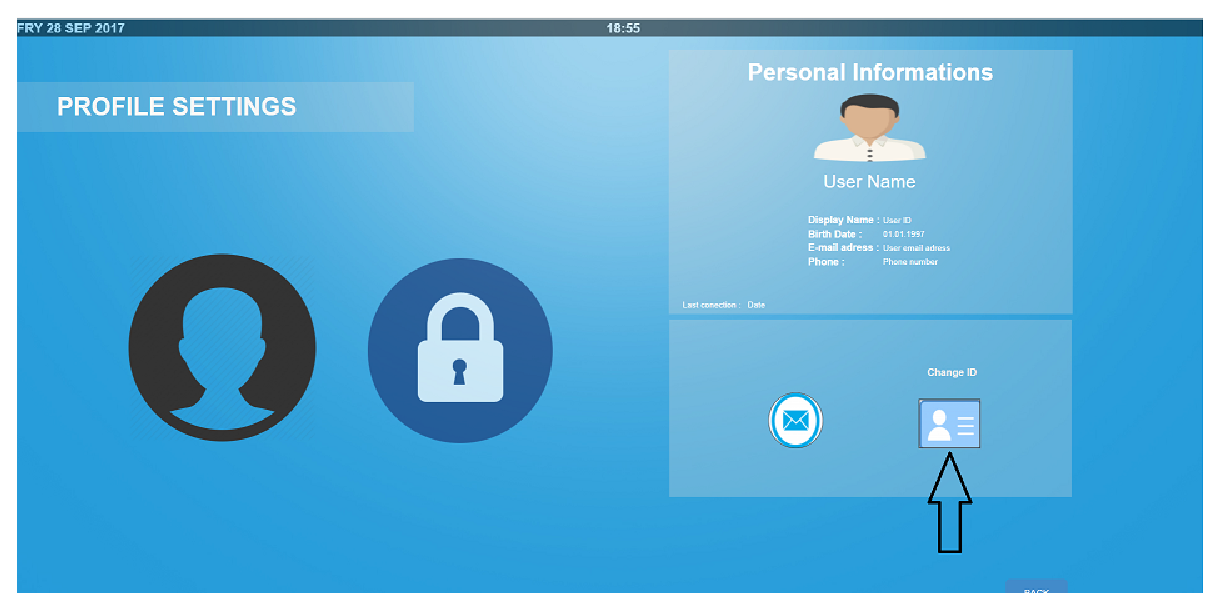
\includegraphics[width=170mm]{images/ChangeID1.eps}
\caption{\label{overflow}}
\end{figure}

\begin{figure}[H]
\centering
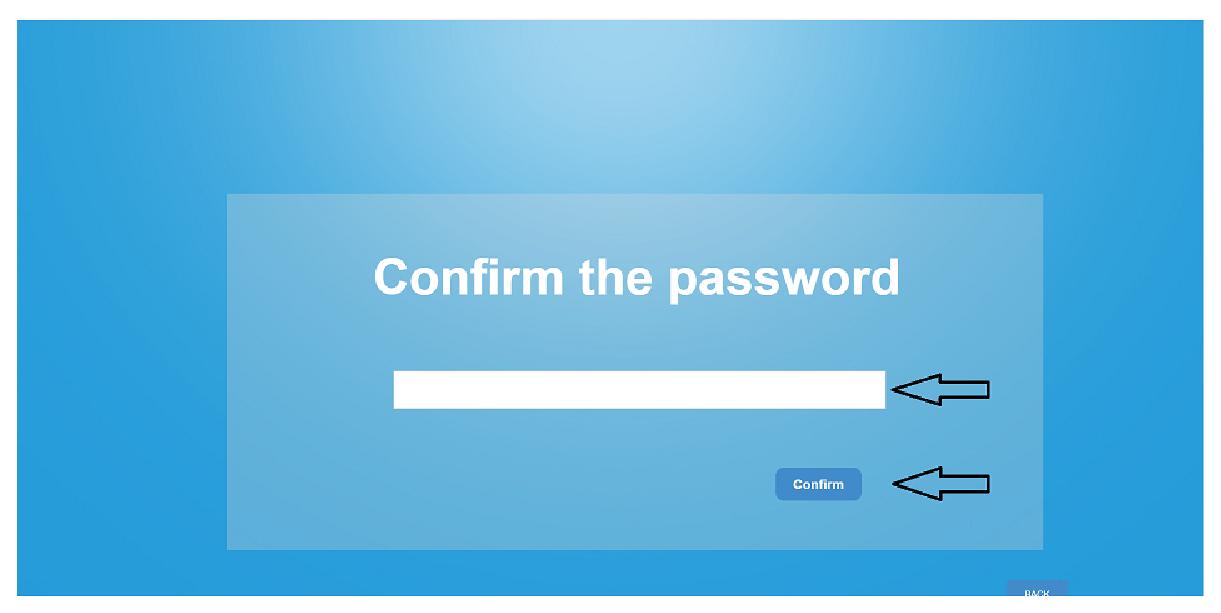
\includegraphics[width=170mm]{images/ComfirmField.eps}
\caption{\label{overflow}}
\end{figure}

\begin{figure}[H]
\centering
\includegraphics[width=170mm]{images/IdField.eps}
\caption{\label{overflow}}
\end{figure}

\begin{figure}[H]
\centering
\includegraphics[width=170mm]{images/IdchangeOk.eps}
\caption{\label{overflow}}
\end{figure}
\end{lyxlist}
\hrule


\subsubsection{Change E-mail}

\hrule
\vspace{0.5cm}
\begin{lyxlist}{PC1}
\small{
\item [\textbf{Procedure:}] ChangeEmail 
\item [\textbf{Scope:}] Allow the super administrator or the SysAdmin to change
their E-mail.
\item [\textbf{Primary Actor}:] SysAdmin Tom
\item [\textbf{Secondary Actor(s)}:] /
\item [\textbf{Goal:}] The SysAdmin Tom should be able to change his E-mail.
\item [\textbf{Level}:] User-goal level
\item [\textbf{Main~Success~Scenario}]:\\
1. \emph{Tom} clicks on the "Change E-mail '' icon in the Account settings
section.\\
2. \emph{Tom} inserts his password in the input text field.\\
3. \emph{Tom} clicks on the ''Confirm'' button to confirm the password.\\
4. \emph{Tom} inserts his new E-mail in the input text field.\\
5. \emph{Tom} clicks on the ''Confirm'' button to change his E-mail.\\
6. \emph The E-mail has been changed and {Tom} clicks on the "ok" button to
terminate the procedure.\\

\item [\textbf{Extensions}]:\\
2.a \emph{Tom} has to be a super-SysAdmin or a SysAdmin and has to be logged in
in order to be able to change his e-mail.\\
}

\begin{figure}[H]
\centering
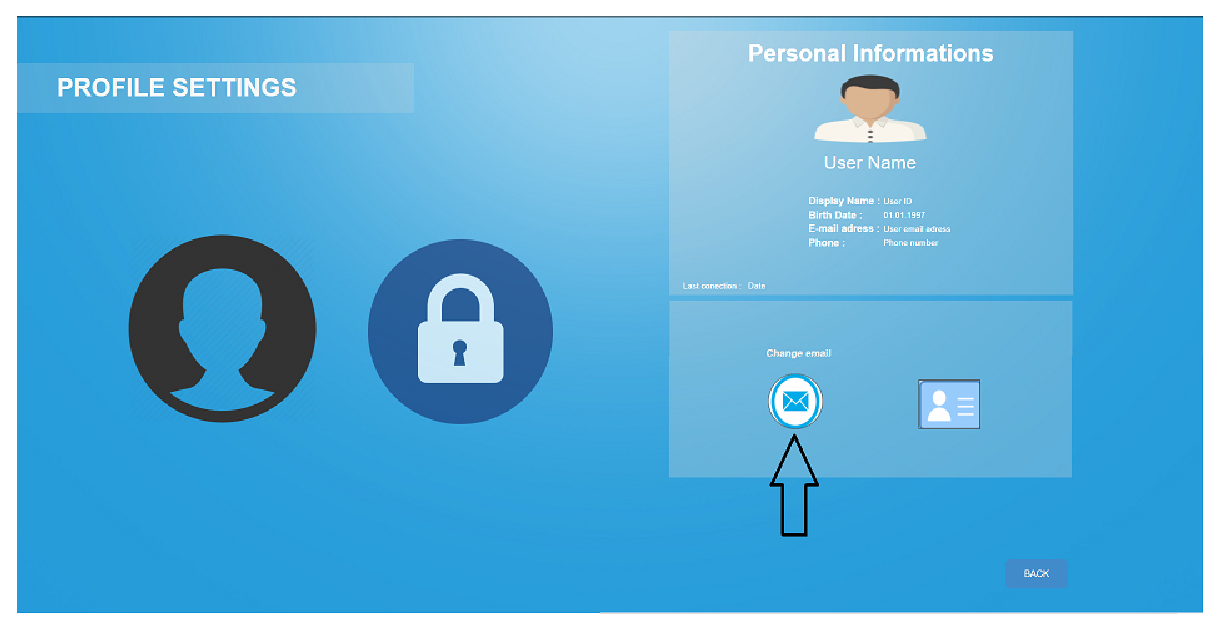
\includegraphics[width=170mm]{images/ChangeEmail1.eps}
\caption{\label{overflow}}
\end{figure}

\begin{figure}[H]
\centering
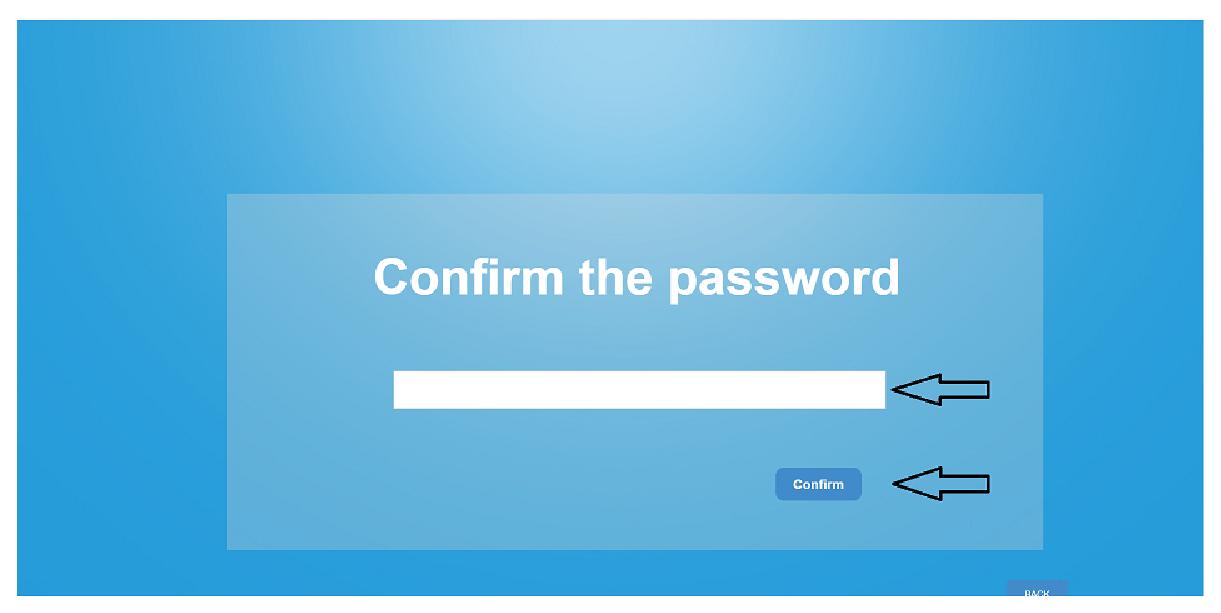
\includegraphics[width=170mm]{images/ComfirmField.eps}
\caption{\label{overflow}}
\end{figure}

\begin{figure}[H]
\centering

\includegraphics[width=170mm]{images/EmailChange1.eps}
\caption{\label{overflow}}
\end{figure}

\begin{figure}[H]
\centering
\includegraphics[width=170mm]{images/EmailChangeOK.eps}
\caption{\label{overflow}}
\end{figure}


\end{lyxlist}
\hrule


\subsubsection{Change Password}

\hrule
\vspace{0.5cm}
\begin{lyxlist}{PC1}
\small{
\item [\textbf{Procedure:}] ChangePassword 
\item [\textbf{Scope:}] Allow the super administrator or the SysAdmin to change
their password.
\item [\textbf{Primary Actor}:] SysAdmin Tom
\item [\textbf{Secondary Actor(s)}:] /
\item [\textbf{Goal:}] The SysAdmin Tom should be able to change his password.
\item [\textbf{Level}:] User-goal level
\item [\textbf{Main~Success~Scenario}]:\\
1. \emph{Tom} clicks on the "Change Password '' icon in the Password settings
section.\\
2. \emph{Tom} inserts his old password in the input text field.\\
3. \emph{Tom} clicks on the ''Confirm'' button to confirm the password.\\
4. \emph{Tom} inserts his new password in the input text field.\\
5. \emph{Tom} clicks on the ''Confirm'' button to change his password.\\
6. \emph The password has been changed and {Tom} clicks on the "ok" button
to terminate the procedure.\\

\item [\textbf{Extensions}]:\\
2.a \emph{Tom} has to be a super-SysAdmin or a SysAdmin and has to be logged in
in order to be able to change his password.\\
}

\begin{figure}[H]
\centering
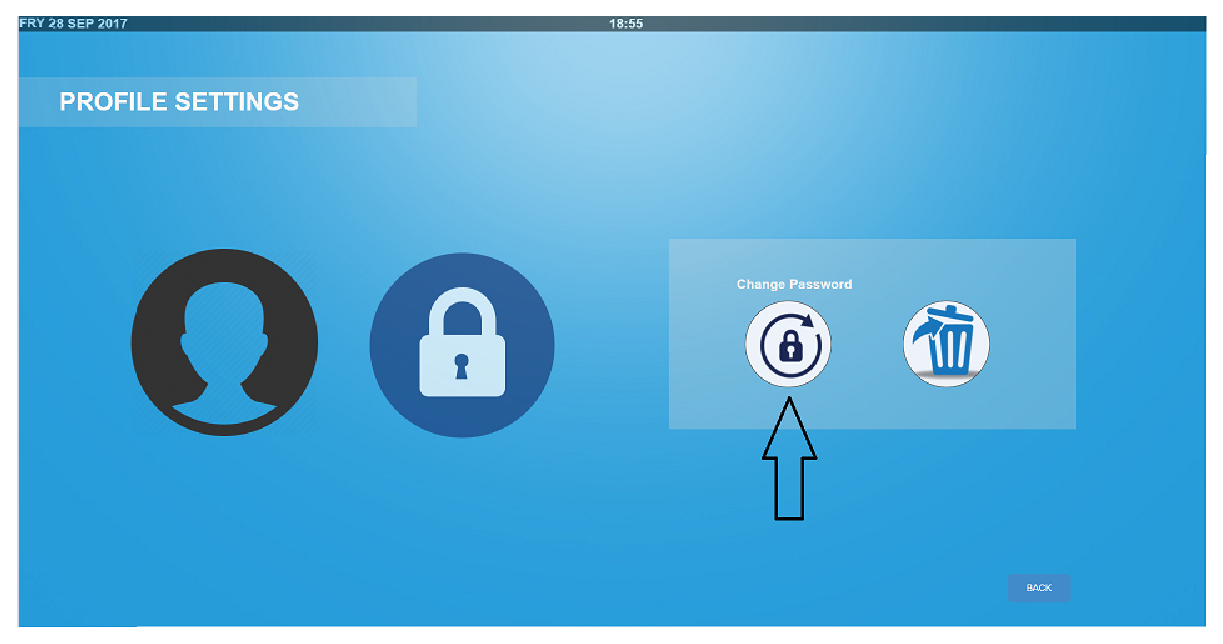
\includegraphics[width=170mm]{images/PasswordChange1.eps}
\caption{\label{overflow}}
\end{figure}

\begin{figure}[H]
\centering
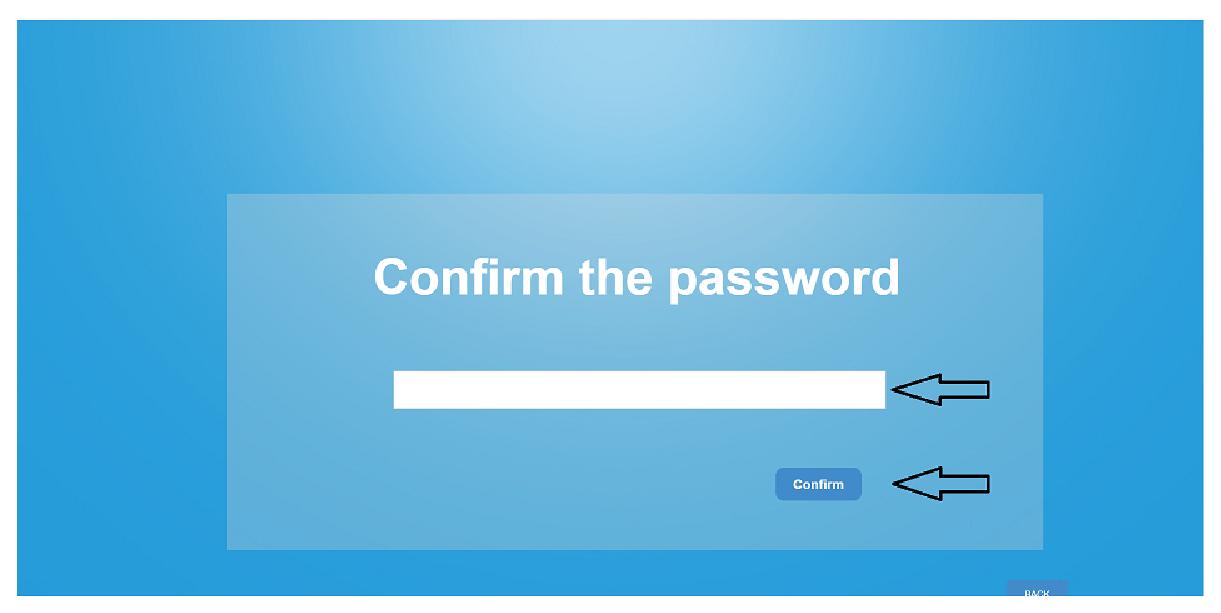
\includegraphics[width=170mm]{images/ComfirmField.eps}
\caption{\label{overflow}}
\end{figure}

\begin{figure}[H]
\centering
\includegraphics[width=170mm]{images/PasswordField1.eps}
\caption{\label{overflow}}
\end{figure}

\begin{figure}[H]
\centering
\includegraphics[width=170mm]{images/PassChangeOk.eps}
\caption{\label{overflow}}
\end{figure}


\end{lyxlist}
\hrule

\section{Mono-procedures}
Mono-procedures must be grouped by actors.





\subsection{SysAdmin}

\subsubsection{Creating a virtual machine using expert mode}

\hrule
\vspace{0.5cm}
\begin{lyxlist}{PC1}
\small{
\item [\textbf{Procedure:}] vmCreationProcess1
\item [\textbf{Scope:}] Virtual machine creation
\item [\textbf{Primary Actor}:] SysAdmin John
\item [\textbf{Secondary Actor(s)}:] /
\item [\textbf{Goal:}] The SysAdmin John should be able to create a virtual
machine which was created with his components that he choosed.
\item [\textbf{Level}:] User-goal level
\item [\textbf{Main~Success~Scenario}]:\\

1. \emph{John} must click on the button 'CREATE VM' in the main Menu.\\
2. \emph{John} must click on the button with a screwdriver called 'OWN
SETTINGS'.\\
3. \emph{John} must enter a name for the virtual machine such as 'JOHNsVM'
and a description 'VM for software engeneering project'.\\
4. \emph{John} must select a CPU 'Intel Xeon E3-1630'.\\
5. \emph{John} must select the CPU amount '2'.\\
6. \emph{John} must click on the right arrow which allows him to
proceed to the next component and the left arrow allows him to go one page
back.\\
7. \emph{John} must select how much does he wants '128GB ECC memory'.\\
8. \emph{John} must select the RAM amount '2'.\\
9. \emph{John} must click on the right arrow which allows him to
proceed to the next component.\\
10. \emph{John} must select a GPU 'NVIDIA QUADRO P4000'.\\
11. \emph{John} must select the GPU amount '2'.\\
12. \emph{John} must click on the right arrow which allows him to
proceed to the next component.\\
13. \emph{John} must select a HDD '4TB 7200 RPM'.\\
14. \emph{John} must select the HDD amount '1'.\\
15. \emph{John} must click on the right arrow which allows him to
proceed to the next component.\\
16. \emph{John} must select a SSD '1 TB SATA SSD'.\\
17. \emph{John} must select the CPU amount '3'.\\
18. \emph{John} must click on the right arrow which allows him to
proceed to the next component.\\
19. \emph{John} must select a SOFTWARE 'SOLIDWORKS'.\\
20. \emph{John} must click on the right arrow which allows him to
proceed to the next component.\\
21. \emph{John} will be at the finish page, here John has now the option to
choose if he wants to create the selected VM, for this he must click on the
green check mark, and if he wants to abandon the configuration he has to
click on the red cross.\\


\item [\textbf{Extensions}]:\\
2.a John has to be logged in, in order to create a virtual machine.







\item [\textbf{GUI screenshot guide}]:\\

}

\begin{figure}[H]
\centering
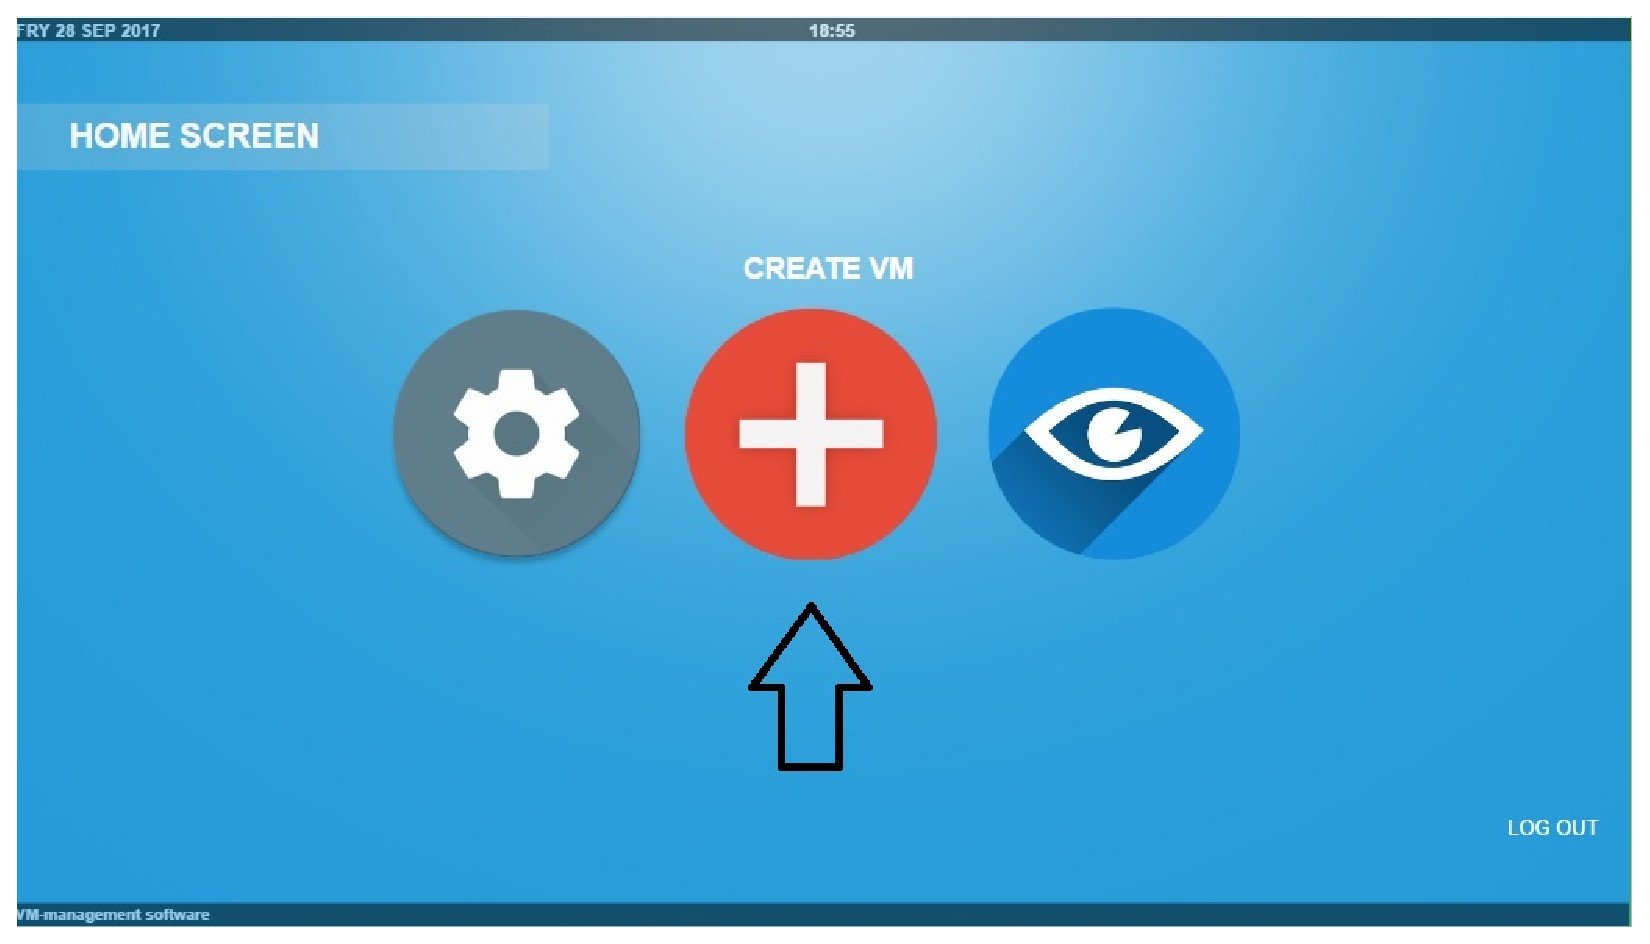
\includegraphics[width=170mm]{images/createVMEx1.eps}
\caption{\label{overflow}}
\end{figure}

\begin{figure}[H]
\centering
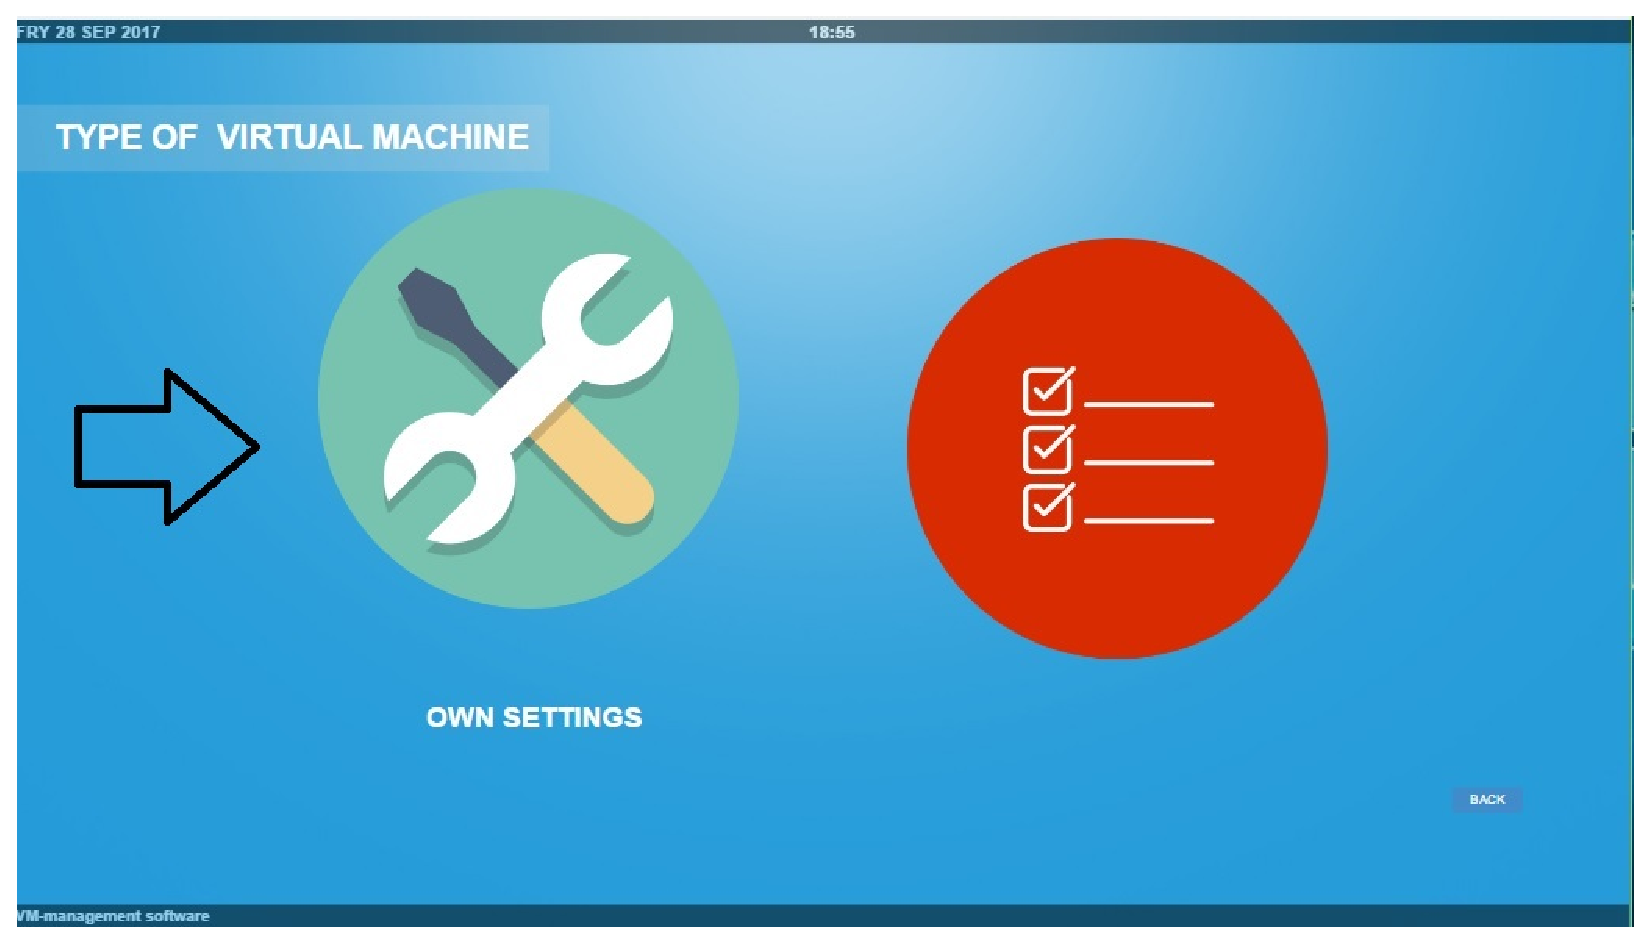
\includegraphics[width=170mm]{images/createVMEx2.eps}
\caption{\label{overflow}}
\end{figure}

\begin{figure}[H]
\centering
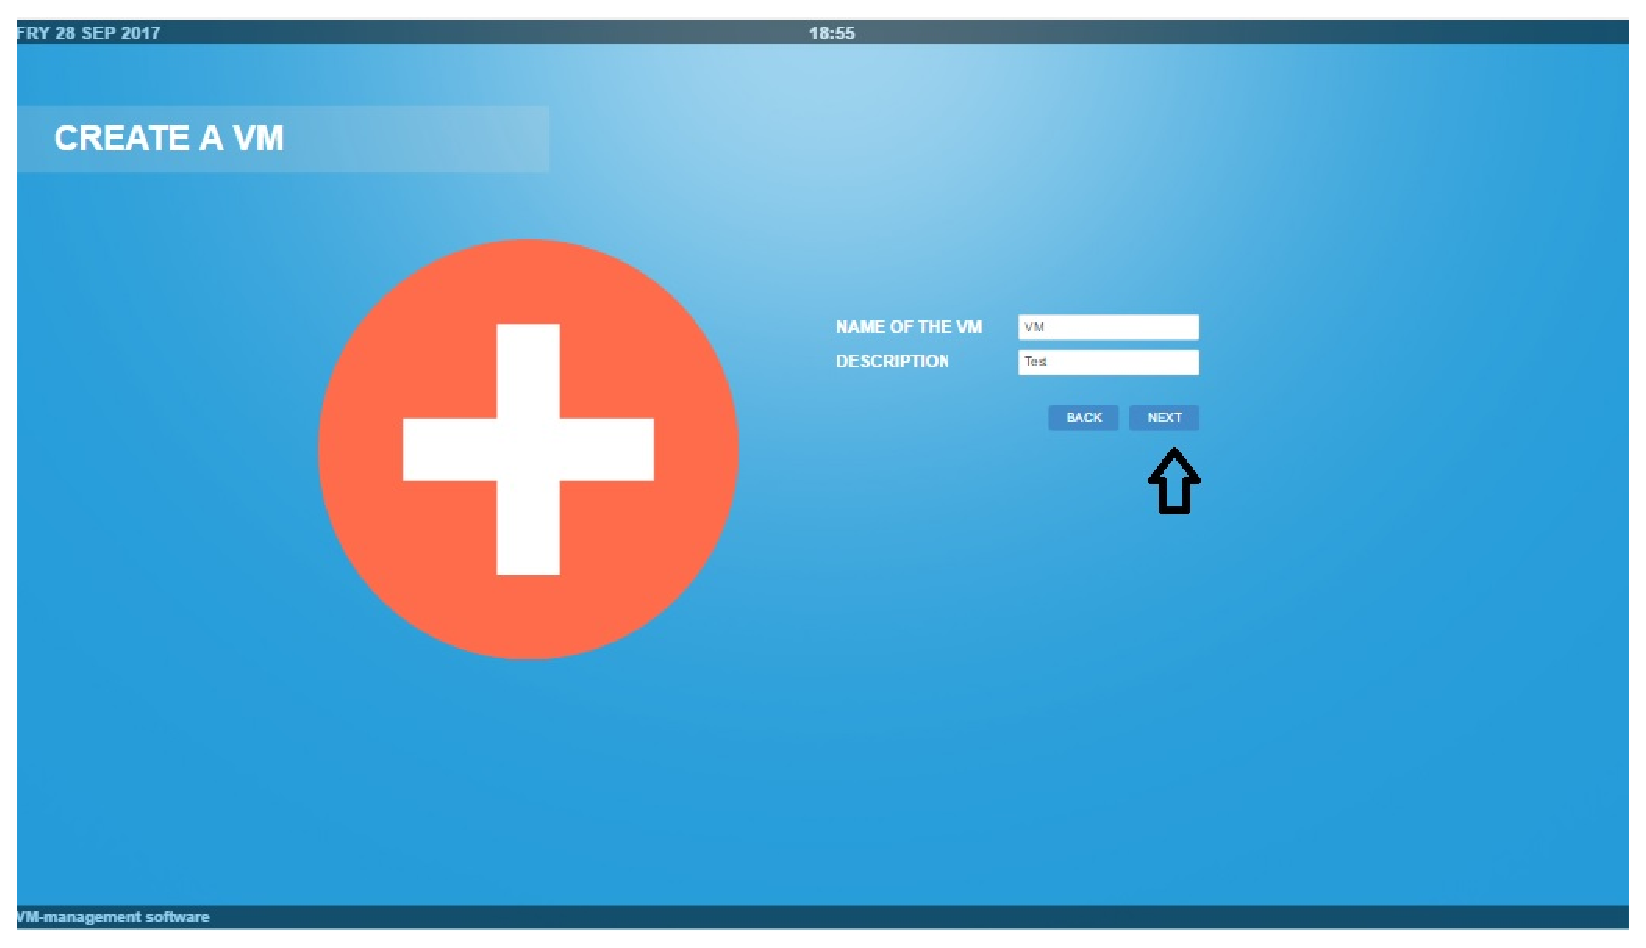
\includegraphics[width=170mm]{images/createVMEx3.eps}
\caption{\label{overflow}}
\end{figure}

\begin{figure}[H]
\centering
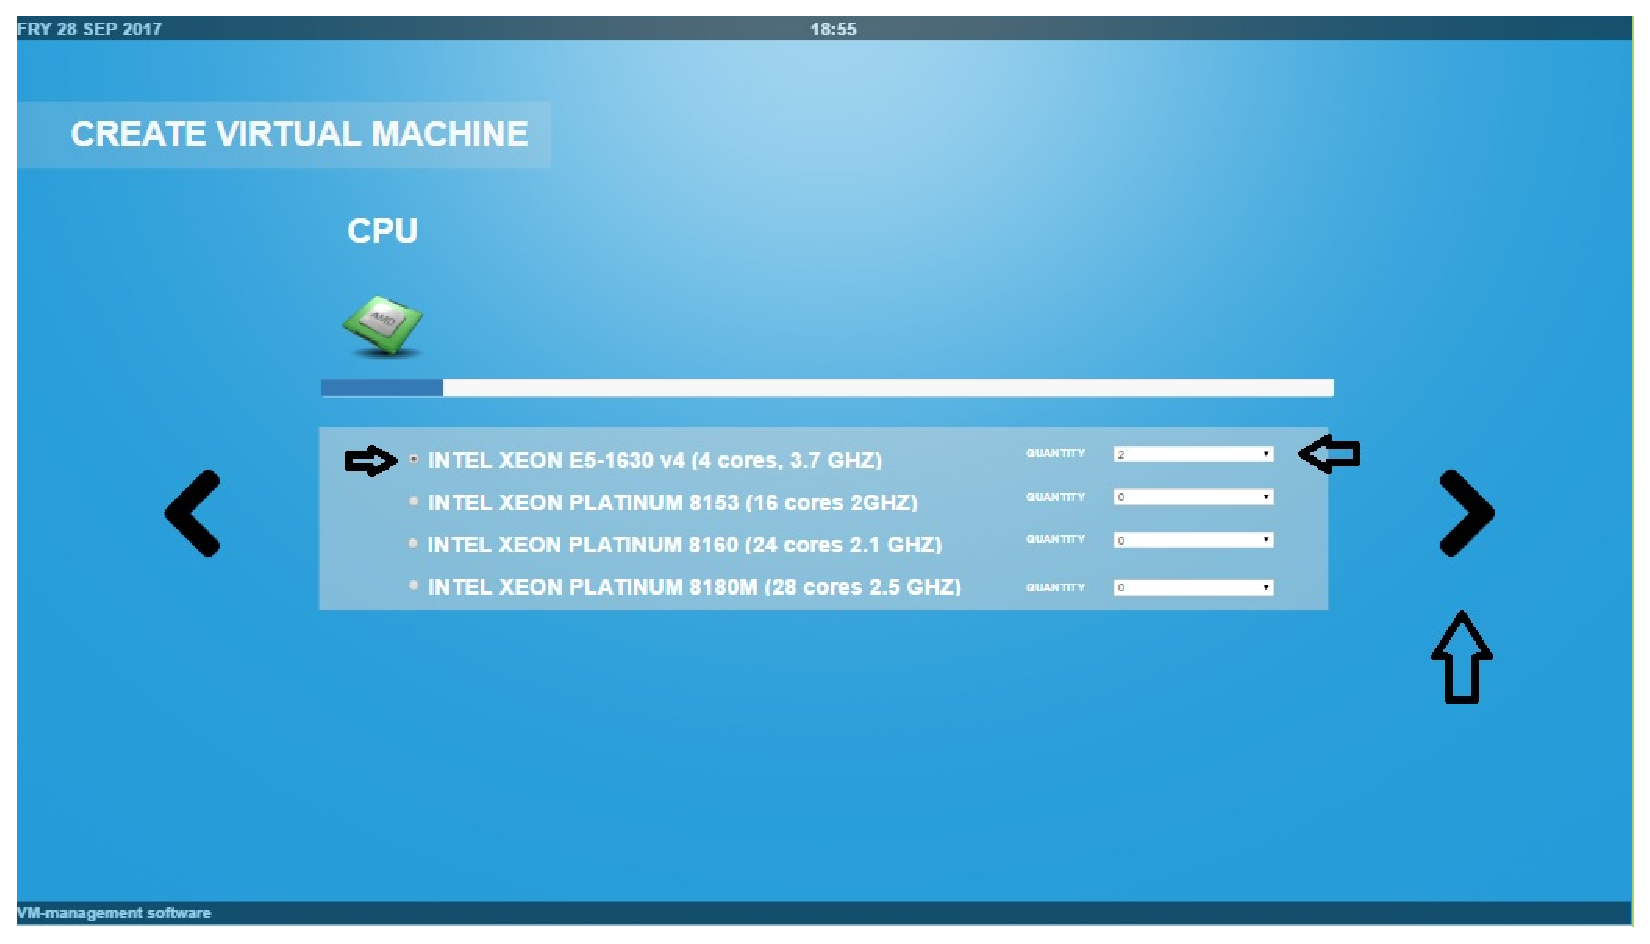
\includegraphics[width=170mm]{images/createVMEx4.eps}
\caption{\label{overflow}}
\end{figure}

\begin{figure}[H]
\centering
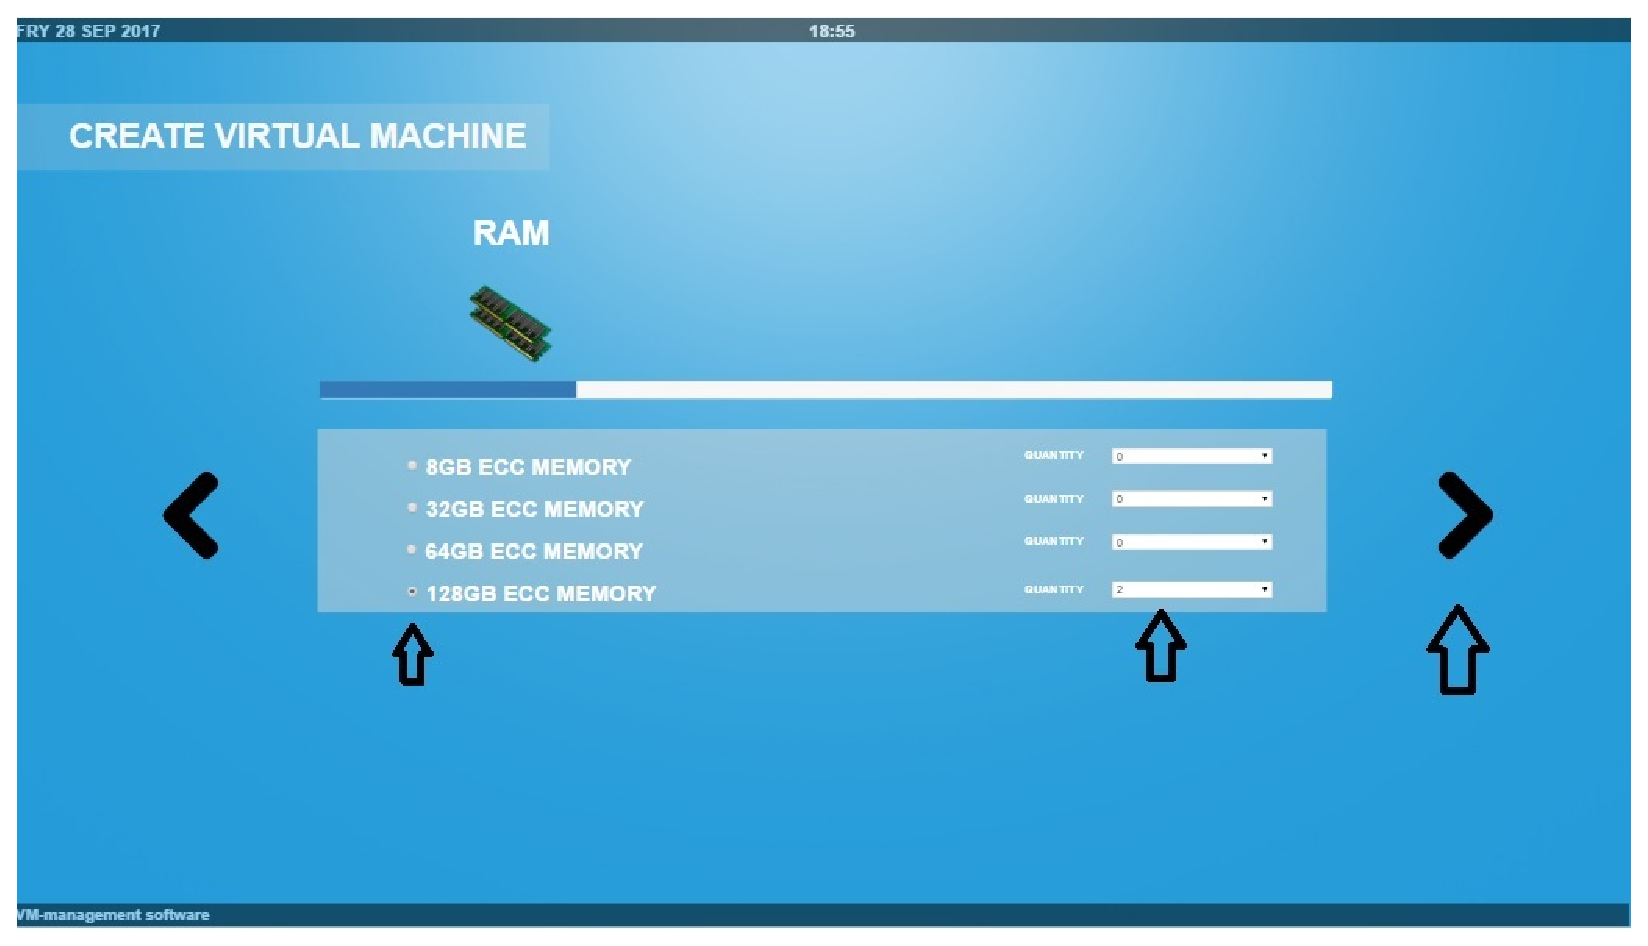
\includegraphics[width=170mm]{images/createVMEx5.eps}
\caption{\label{overflow}}
\end{figure}

\begin{figure}[H]
\centering
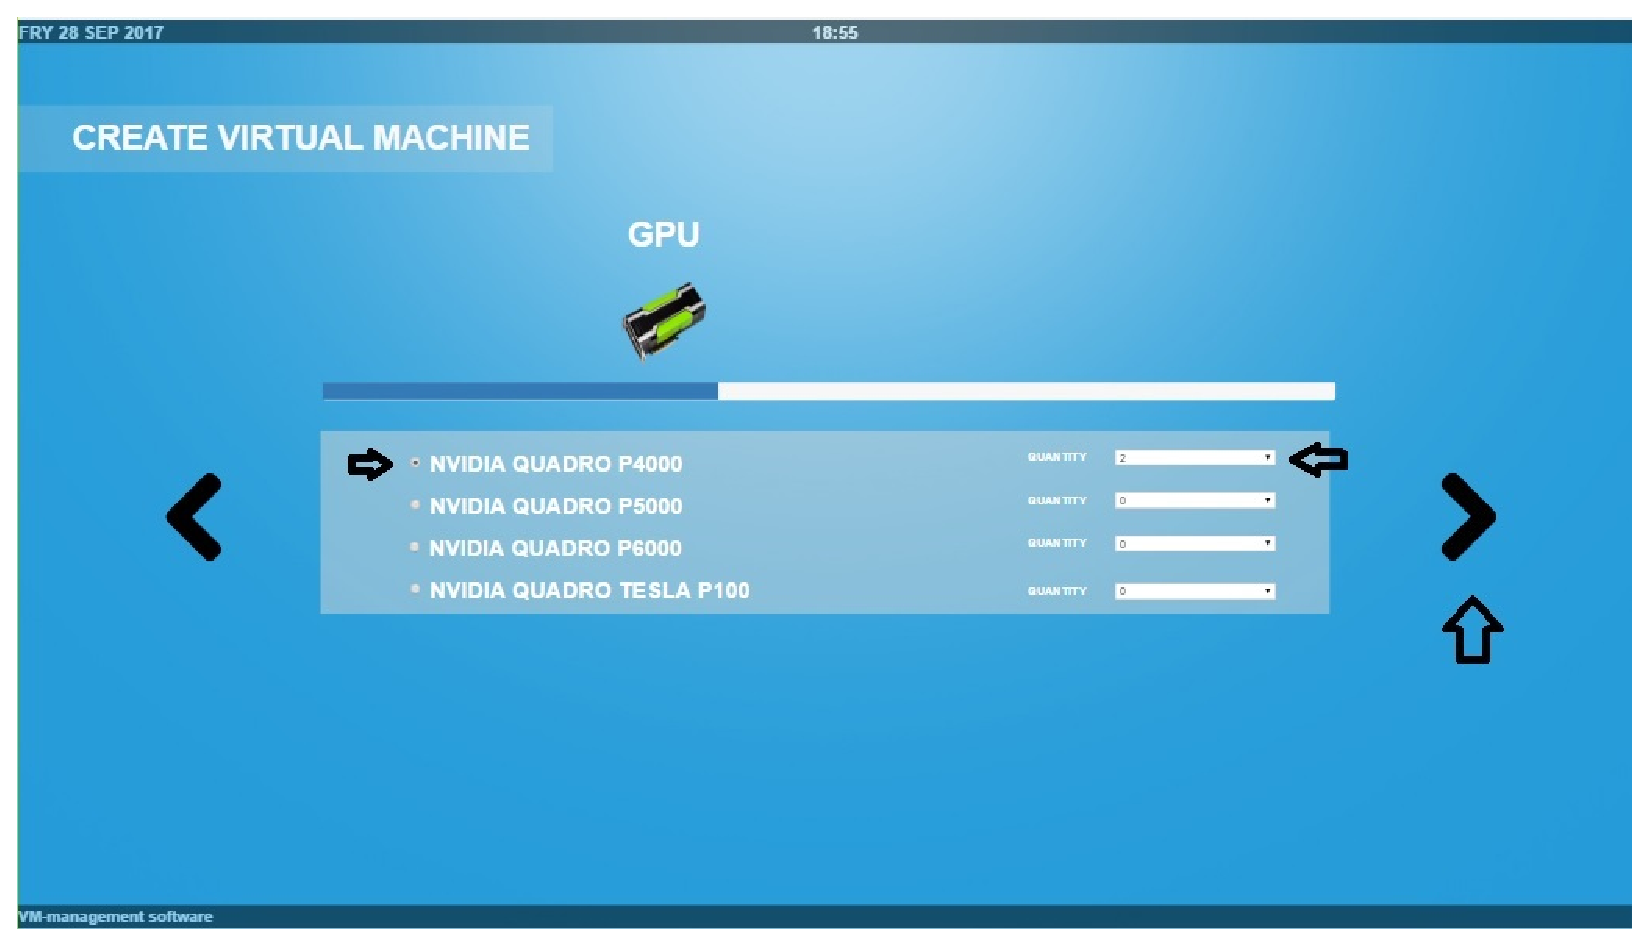
\includegraphics[width=170mm]{images/createVMEx6.eps}
\caption{\label{overflow}}
\end{figure}

\begin{figure}[H]
\centering
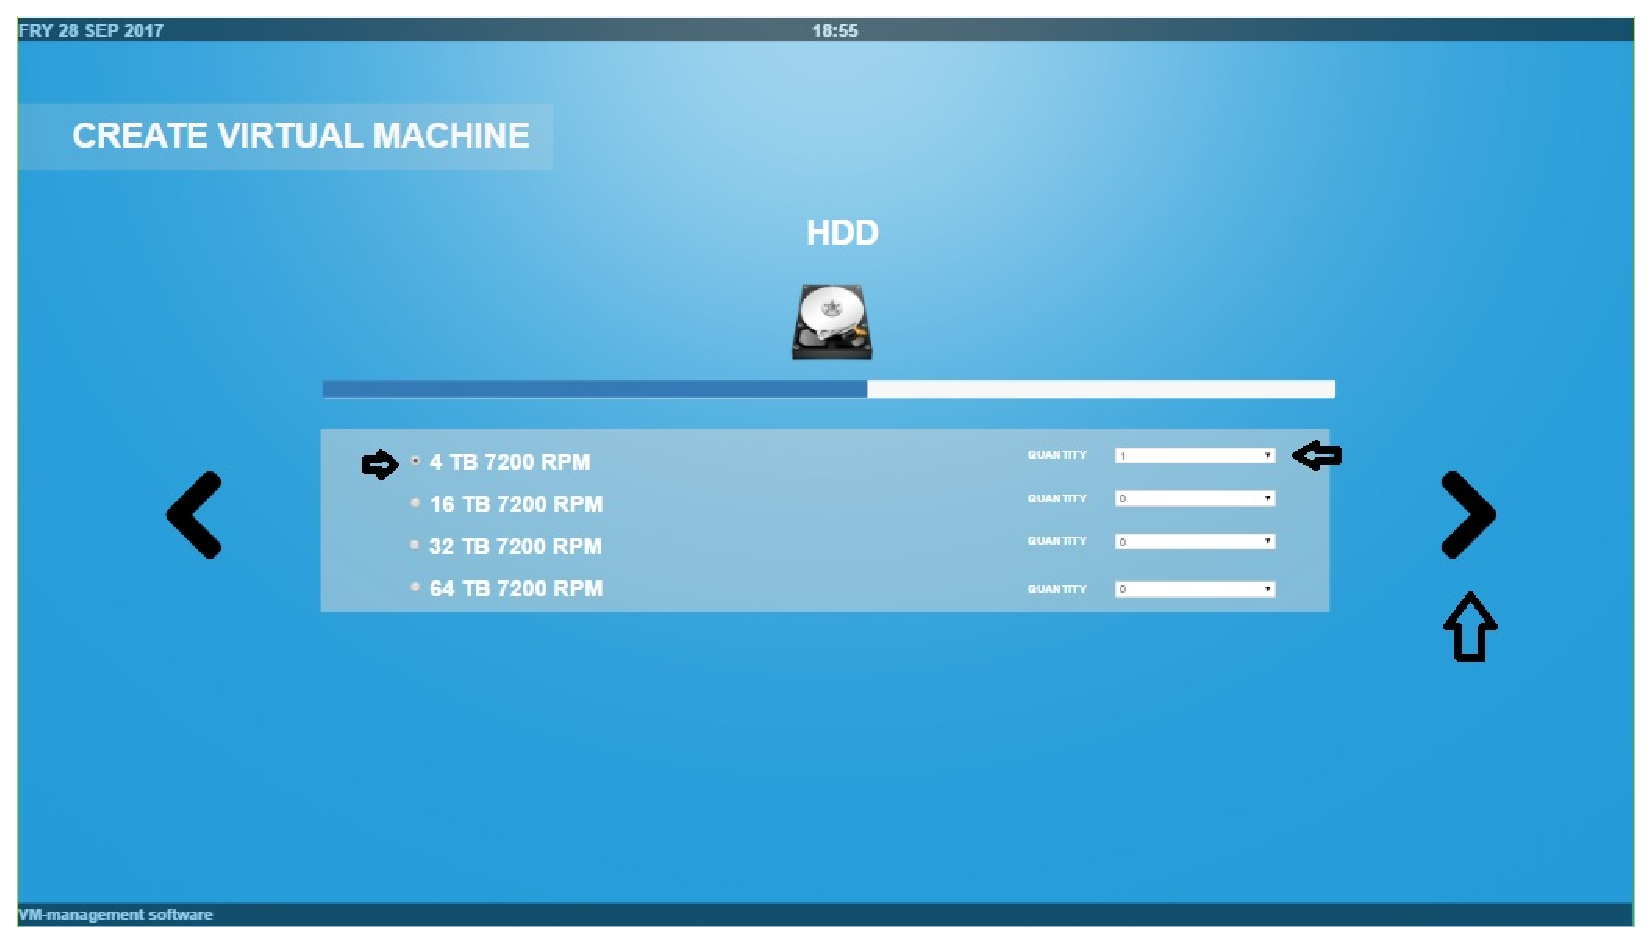
\includegraphics[width=170mm]{images/createVMEx7.eps}
\caption{\label{overflow}}
\end{figure}

\begin{figure}[H]
\centering
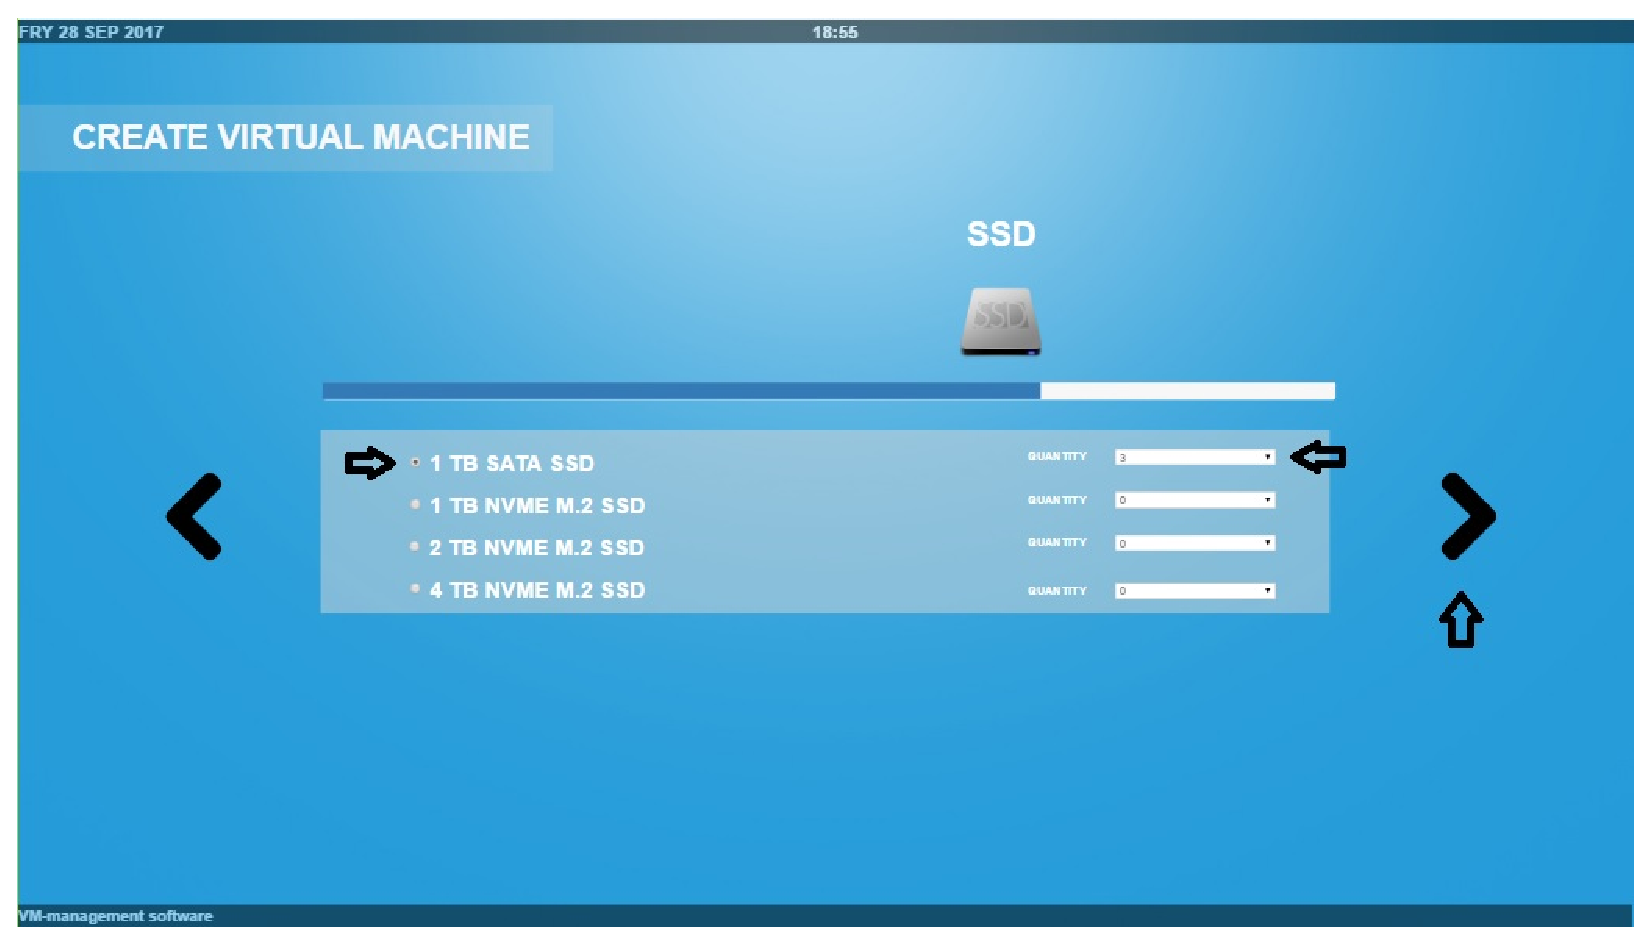
\includegraphics[width=170mm]{images/createVMEx8.eps}
\caption{\label{overflow}}
\end{figure}

\begin{figure}[H]
\centering
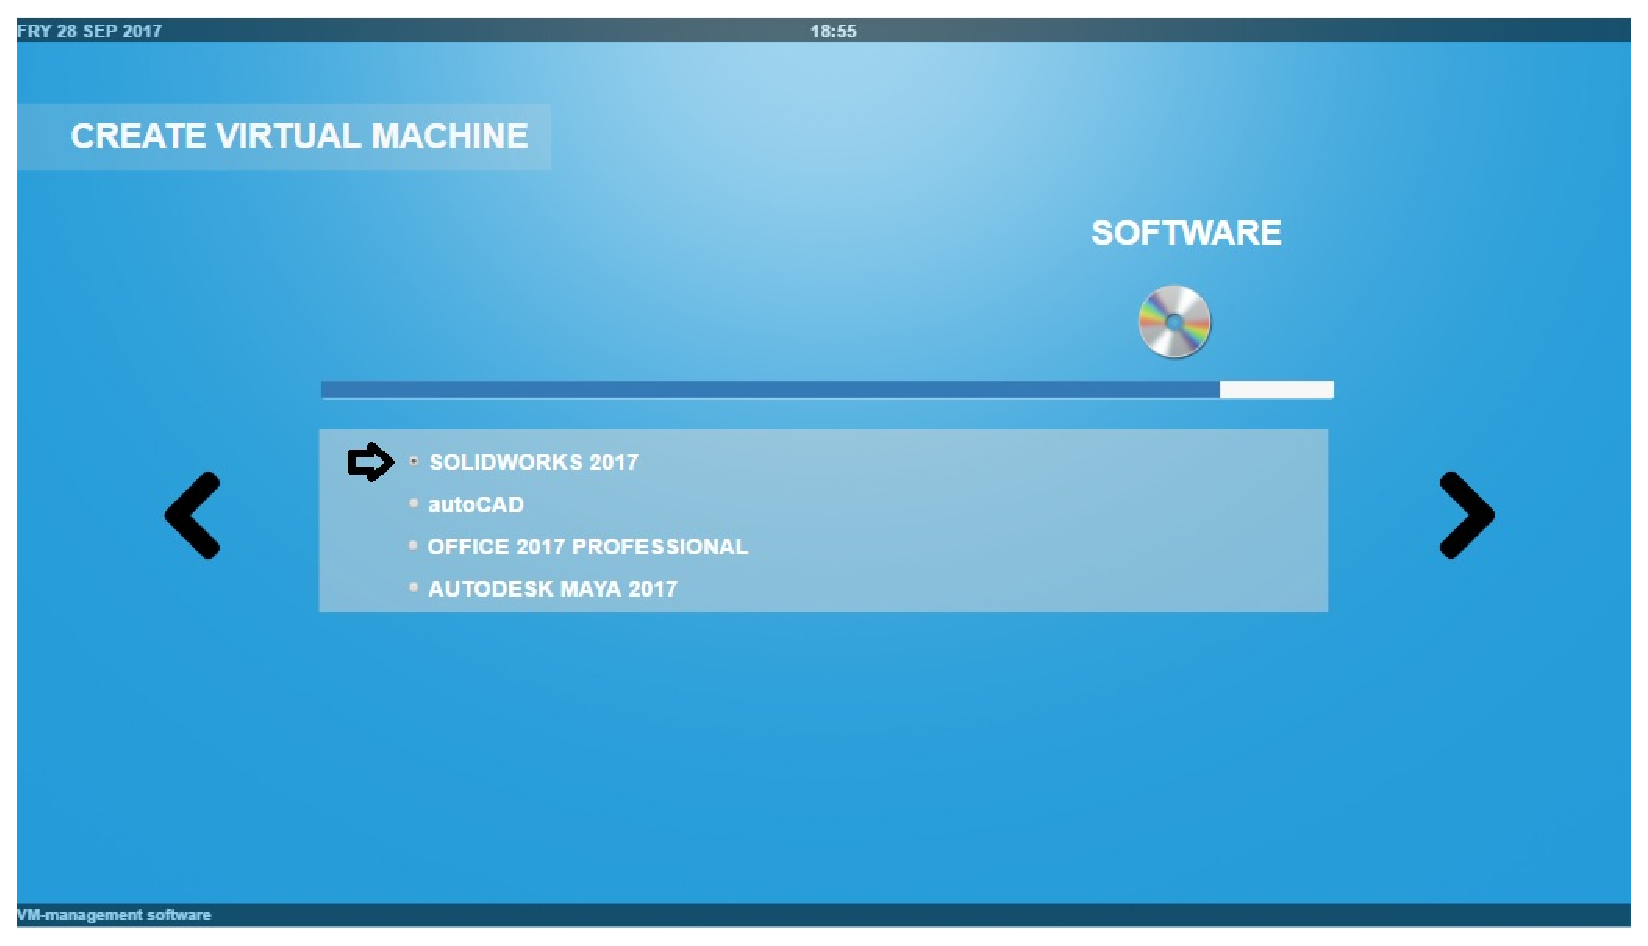
\includegraphics[width=170mm]{images/createVMEx9.eps}
\caption{\label{overflow}}
\end{figure}

\begin{figure}[H]
\centering
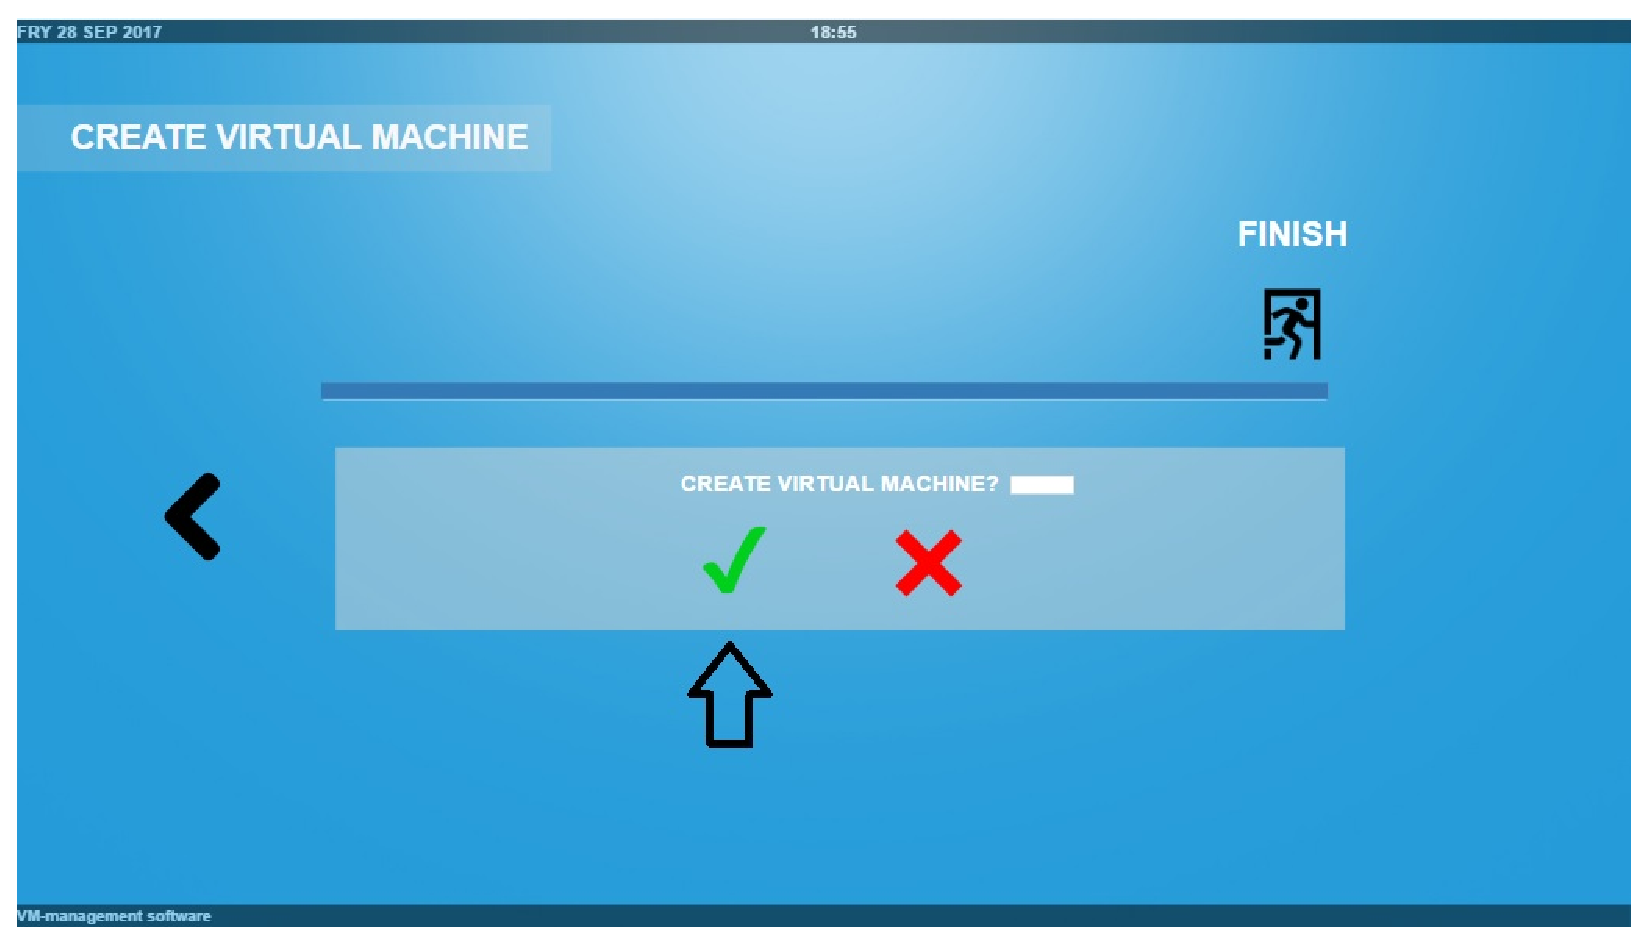
\includegraphics[width=170mm]{images/createVMEx10.eps}
\caption{\label{overflow}}
\end{figure}

\end{lyxlist}
\hrule
\vspace{0.5cm}





\subsubsection{Creating a virtual machine using templates}

\hrule
\vspace{0.5cm}
\begin{lyxlist}{PC1}
\small{
\item [\textbf{Procedure:}] vmCreationProcess2
\item [\textbf{Scope:}] Virtual machine creation
\item [\textbf{Primary Actor}:] SysAdmin John 
\item [\textbf{Secondary Actor(s)}:] /
\item [\textbf{Goal:}] The SysAdmin John should be able to create a virtual
machine which was created using a template.
\item [\textbf{Level}:] User-goal level
\item [\textbf{Main~Success~Scenario}]:\\
1. \emph{John} must click on the button "CREATE VM" in the main
Menu.\\
2. \emph{John} must click on the red button called 'PREDIFINED TEMPLATES'.\\ 
3. \emph{John} must enter a name for his virtual machine 'JOHN'sTEMPLATEVM' and
a description 'VM for software engeneering project'.\\
4. \emph{John} must click on the button named 'NEXT'.\\
5. \emph{John} must answer the different questions with 'YES' or 'NO'.\\
6. \emph{John} must click on button called 'NEXT' and wait a couple of
seconds.\\
7. \emph{John} will see a preconfigured template that perfectly
matches his needs.\\
8. \emph{John} must click on the button called 'FINISH' to accept.\\


\item [\textbf{Extensions}]:\\
2.a John has to be logged in, in order to create a virtual machine.

\item [\textbf{GUI screenshot guide}]:\\
}

\begin{figure}[H]
\centering
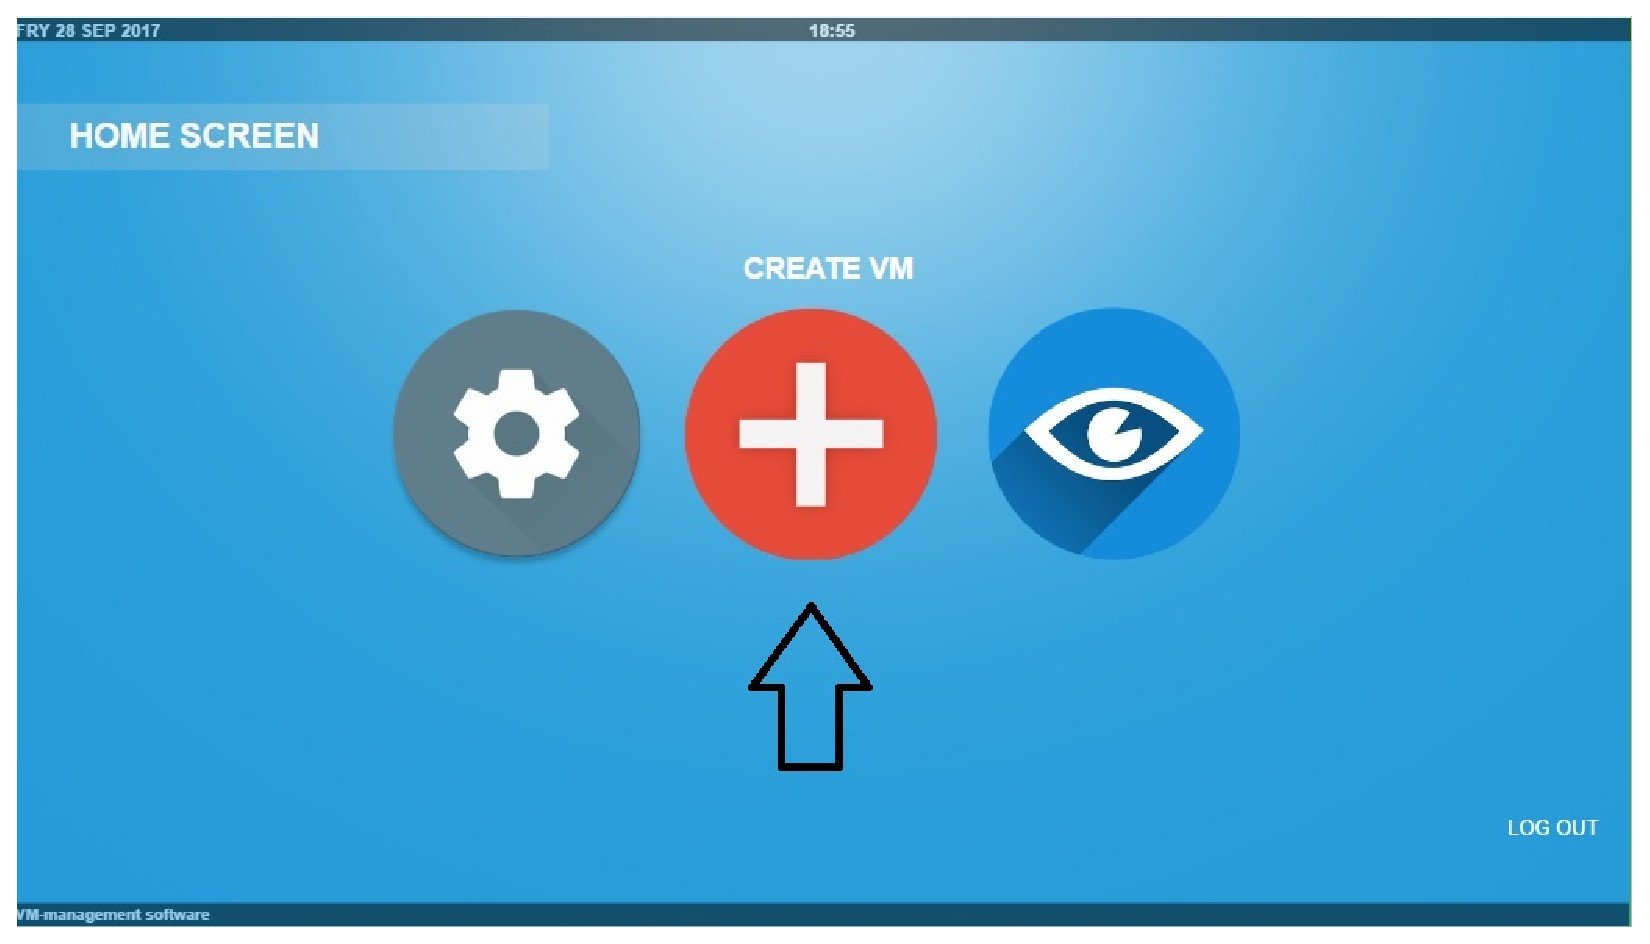
\includegraphics[width=170mm]{images/createVMEx1.eps}
\caption{\label{overflow}}
\end{figure}


\begin{figure}[H]
\centering
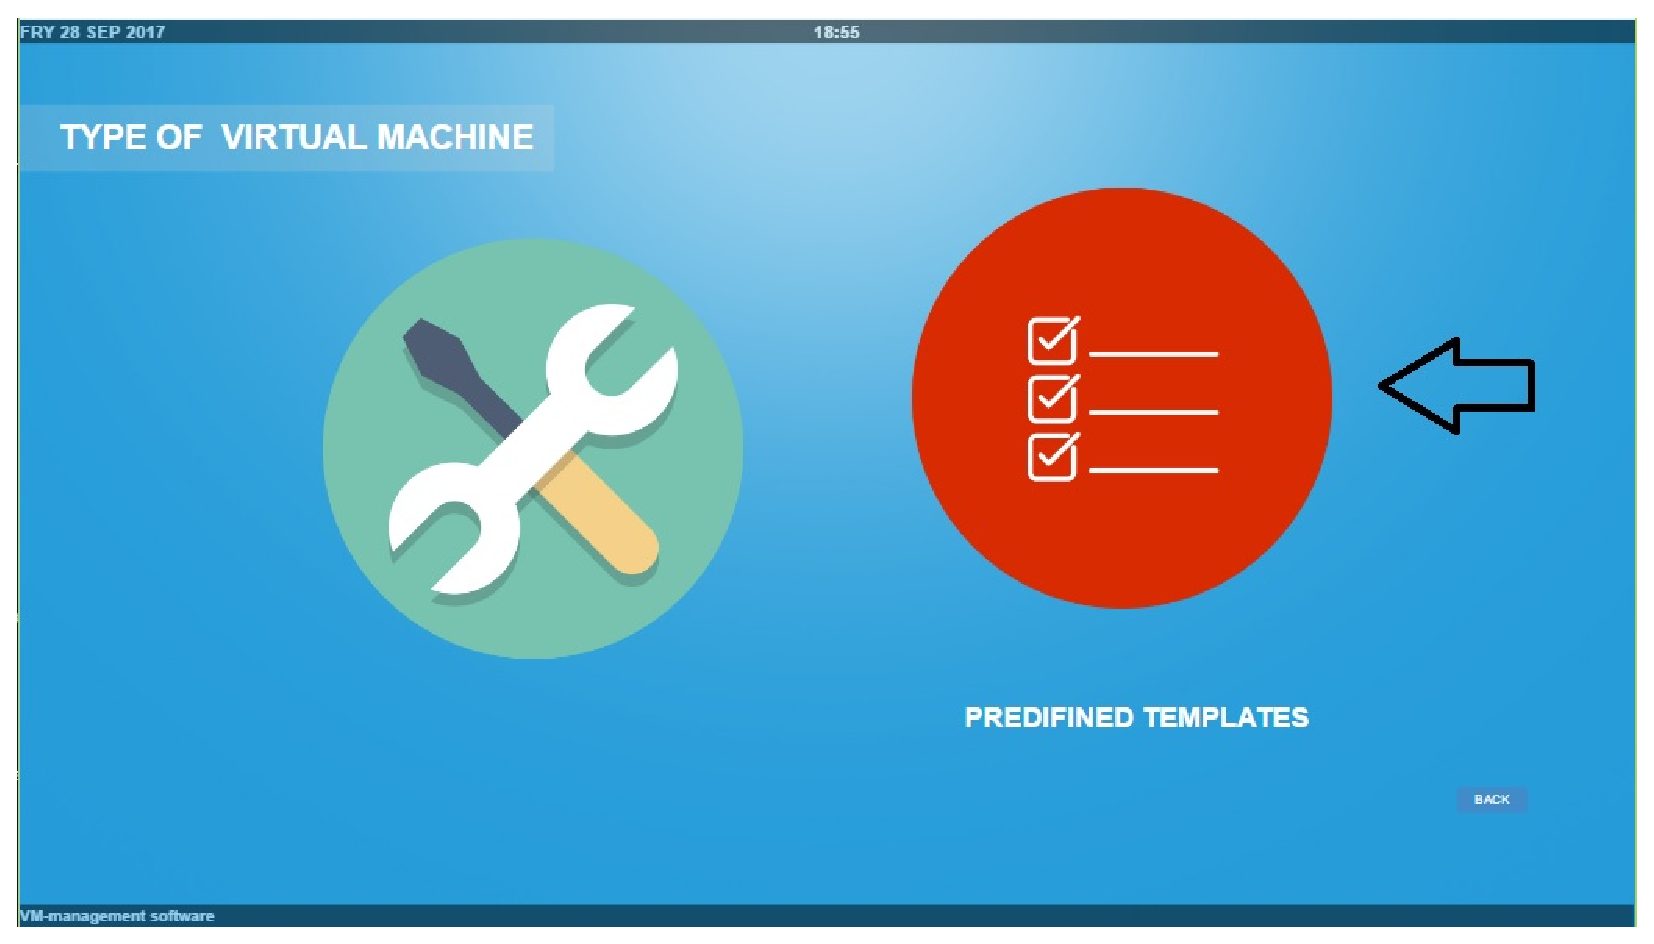
\includegraphics[width=170mm]{images/createVMTemp2.eps}
\caption{\label{overflow}}
\end{figure}

\begin{figure}[H]
\centering
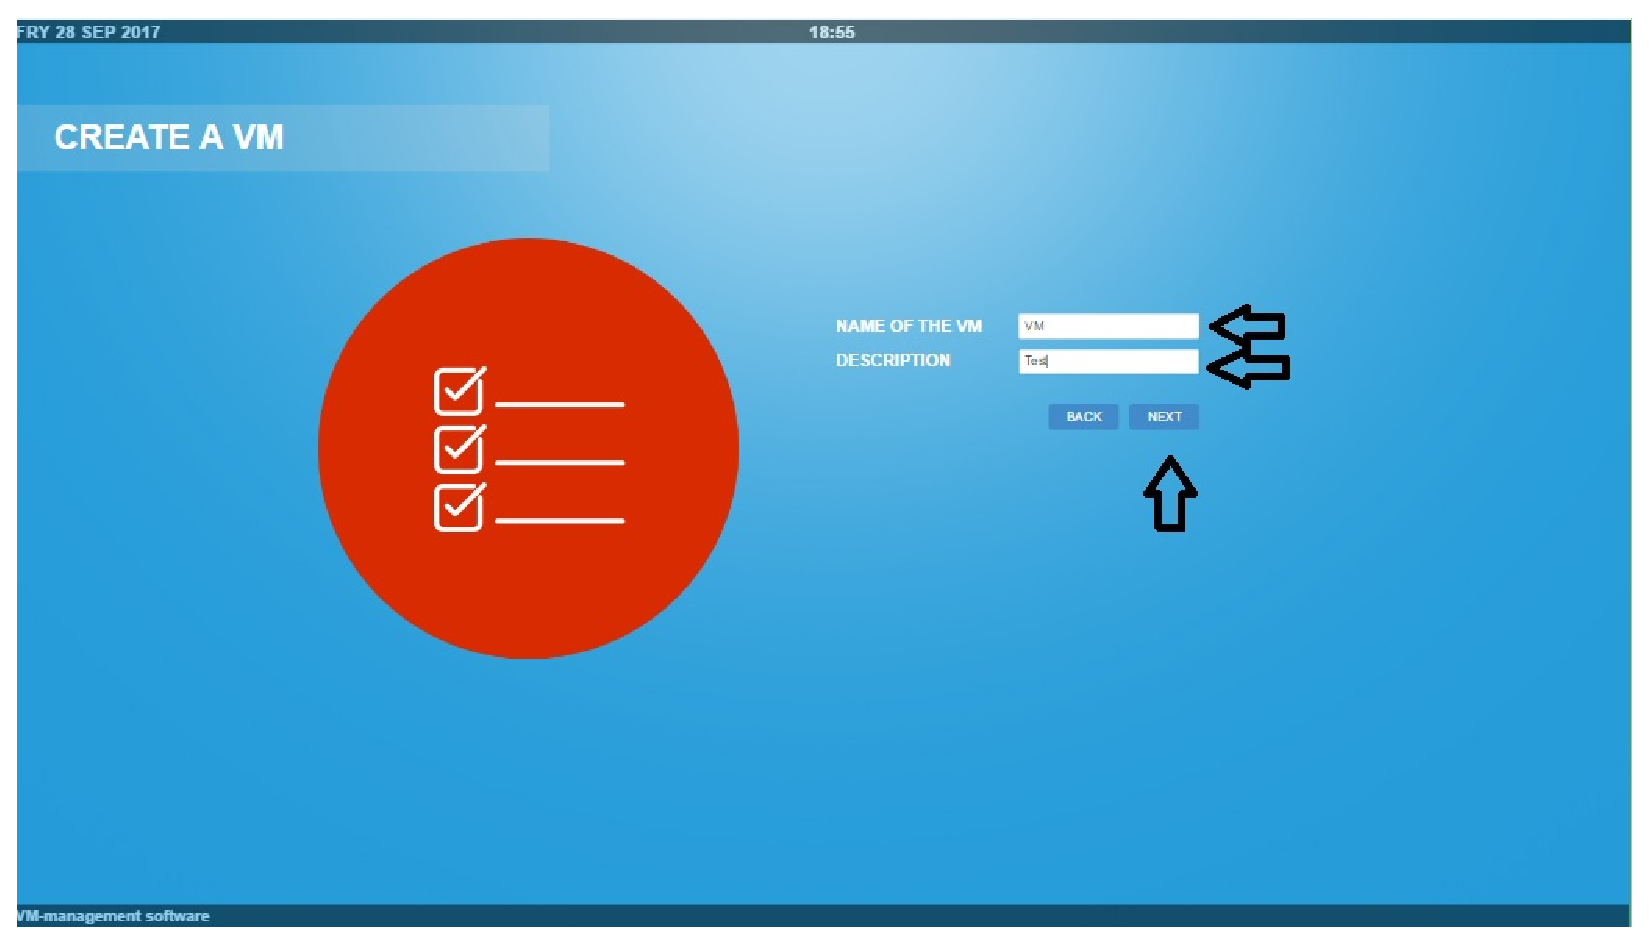
\includegraphics[width=170mm]{images/createVMTemp3.eps}
\caption{\label{overflow}}
\end{figure}

\begin{figure}[H]
\centering
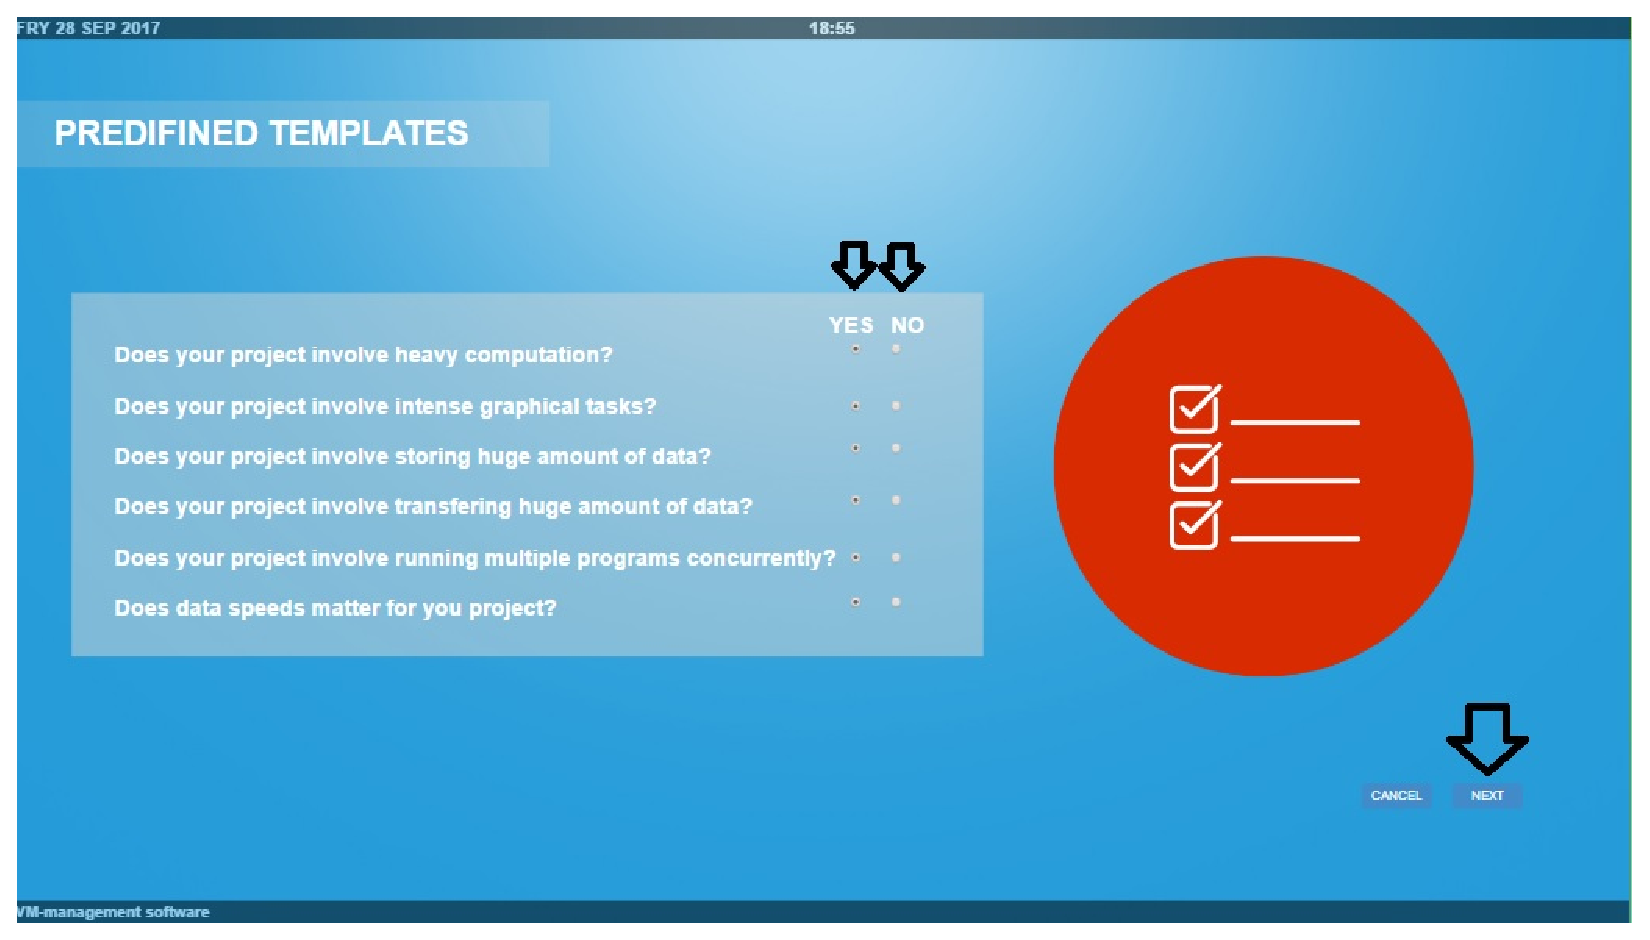
\includegraphics[width=170mm]{images/createVMTemp4.eps}
\caption{\label{overflow}}
\end{figure}


\begin{figure}[H]
\centering
\includegraphics[width=170mm]{images/createVMTemp5.eps}
\caption{\label{overflow}}
\end{figure}

\end{lyxlist}
\hrule
\vspace{0.5cm}








\subsubsection{Modifying a virtual machine}

\hrule
\vspace{0.5cm}
\begin{lyxlist}{PC1}
\small{
\item [\textbf{Procedure:}] vmModificationProcess
\item [\textbf{Scope:}] Virtual machine modification
\item [\textbf{Primary Actor}:] SysAdmin John 
\item [\textbf{Secondary Actor(s)}:] /
\item [\textbf{Goal:}] The SysAdmin John should be able to modify the CPU of
his virtual machine which \emph{John} created before.
\item [\textbf{Level}:] User-goal level
\item [\textbf{Main~Success~Scenario}]:\\
1. \emph{John} must click on the button "VIEW VM's" in the main Menu.\\
2. \emph{John} will see all the virtual machines that he created.\\
3. \emph{John} must select a virtual machine 'JOHN'sVM' and click on it.\\
4. \emph{John} must click now on the left button named `MODIFY`.\\
5. \emph{John} must now choose which components he wants to modify.\\
6. \emph{John} wants to change his CPU so \emph{John} will select the new CPU
'Intel XEON PLATINUM 8180M'.\\
7. \emph{John} must click on the right black arrow to proceed to the next
component. \\
8. \emph{John} must repeat step 6 until he arrives at the finish page.\\
9. \emph{John} must now accept the modification(s) by clicking on the green
check mark.\\


\item [\textbf{Extensions}]:\\
2.a John has to be logged in, in order to create a virtual machine.\\
2.b John must have created at least one virtual machine before, in case to
perform a modification.\\

\item [\textbf{GUI screenshot guide}]:\\
}


\begin{figure}[H]
\centering
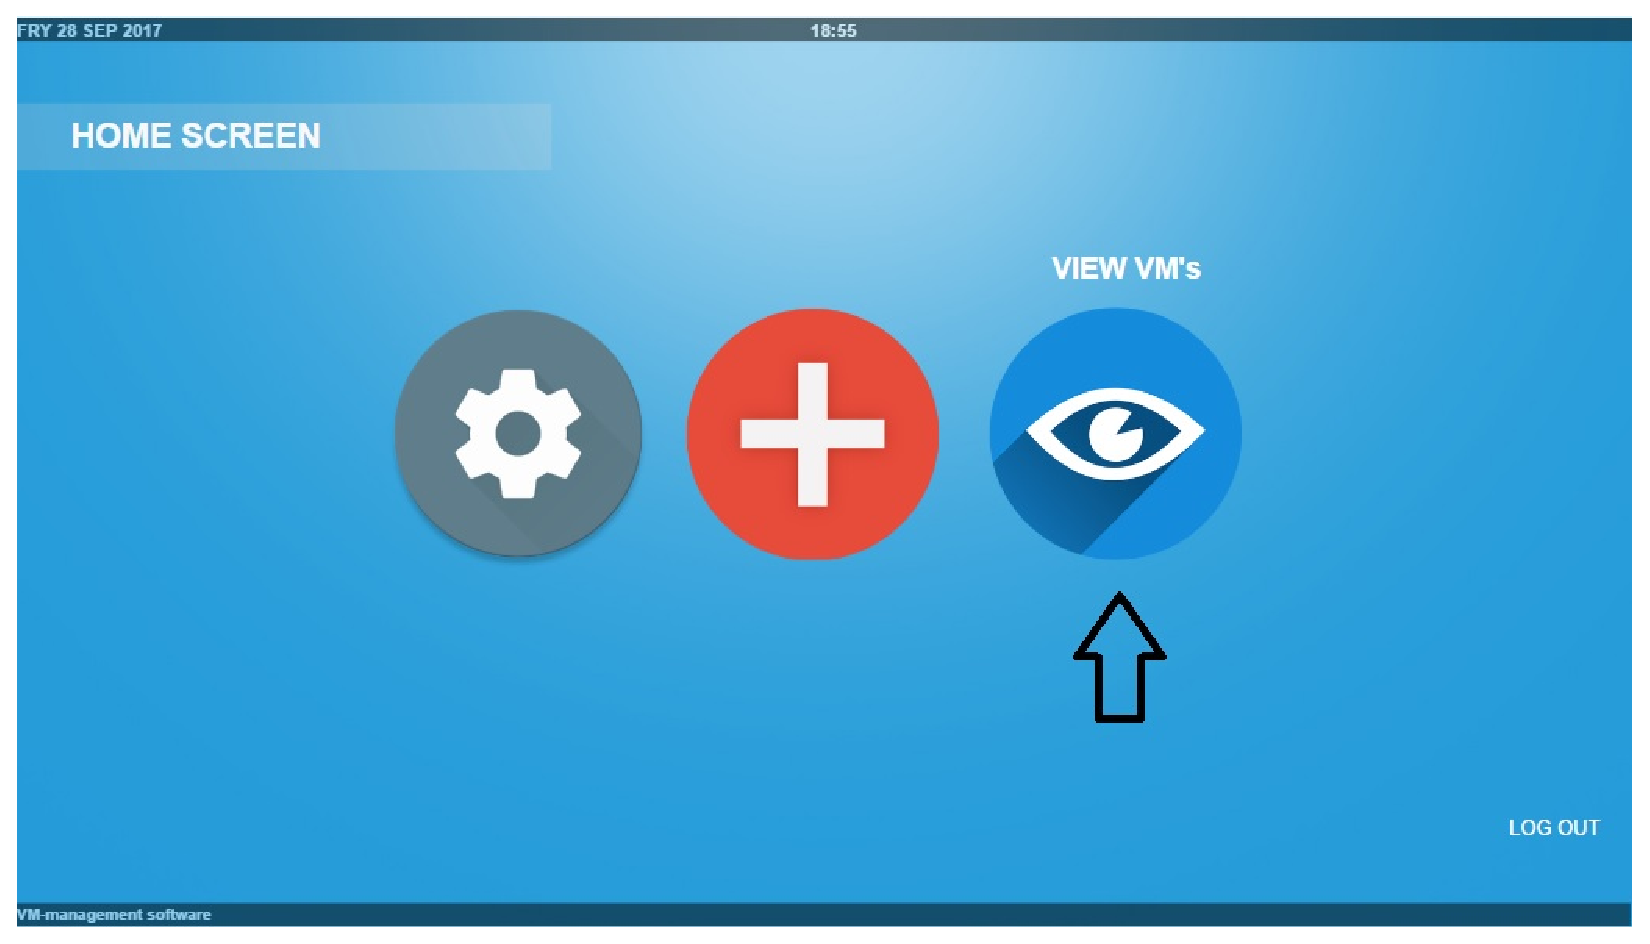
\includegraphics[width=170mm]{images/createVMMod1.eps}
\caption{\label{overflow}}
\end{figure}


\begin{figure}[H]
\centering
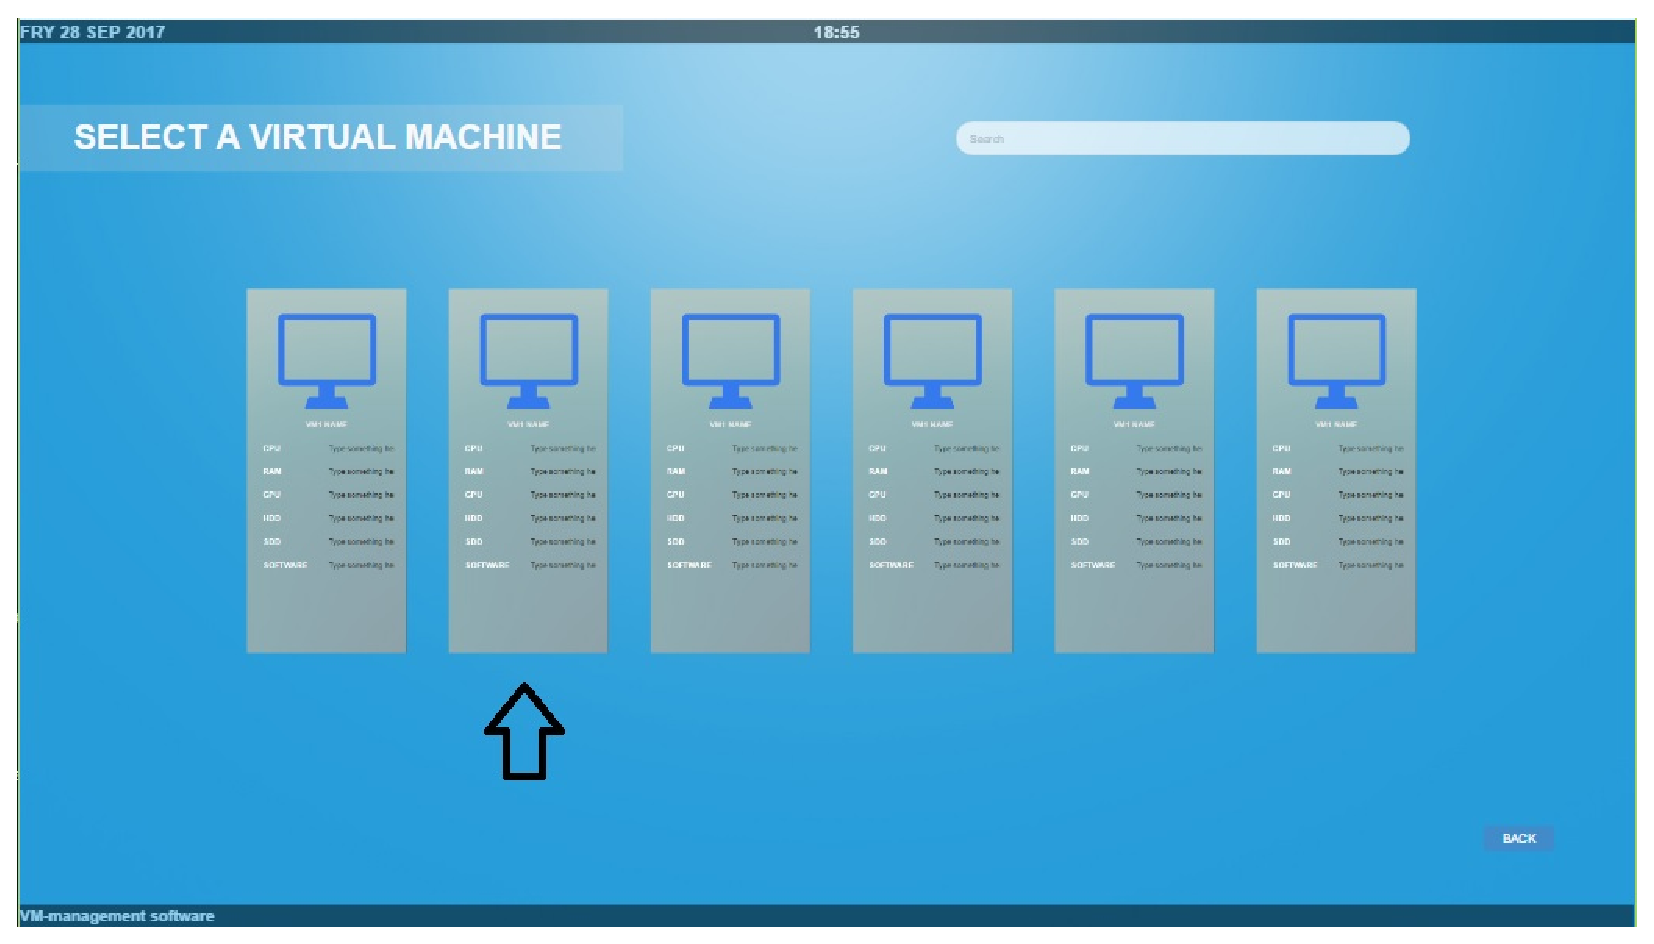
\includegraphics[width=170mm]{images/createVMMod2.eps}
\caption{\label{overflow}}
\end{figure}

\begin{figure}[H]
\centering
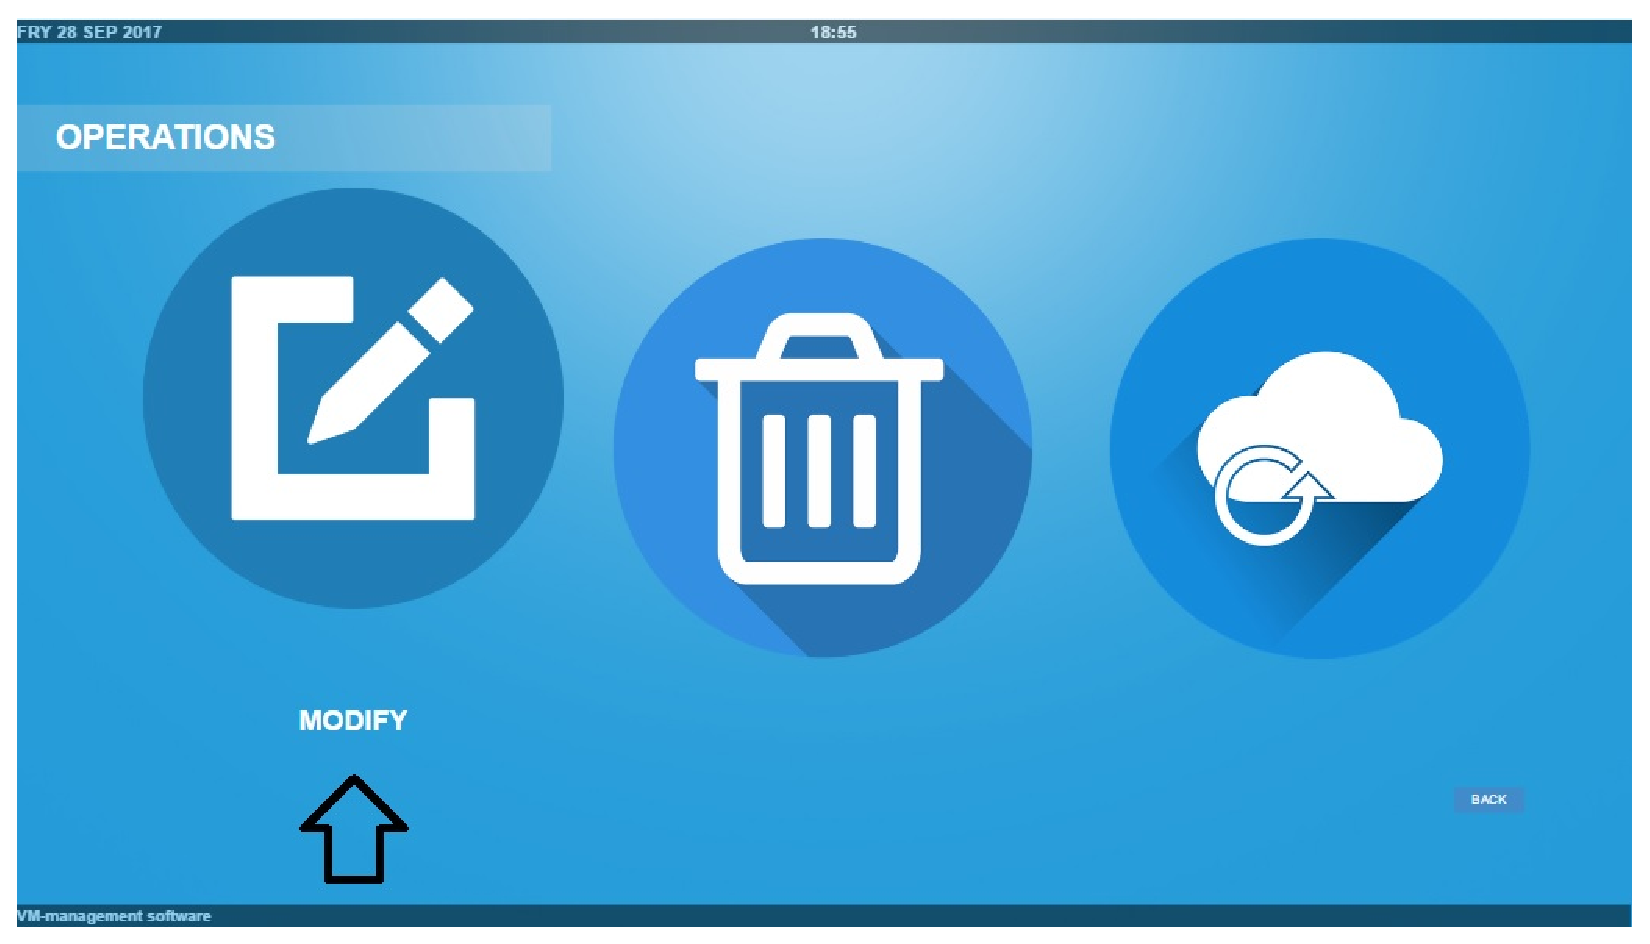
\includegraphics[width=170mm]{images/createVMMod3.eps}
\caption{\label{overflow}}
\end{figure}

\begin{figure}[H]
\centering
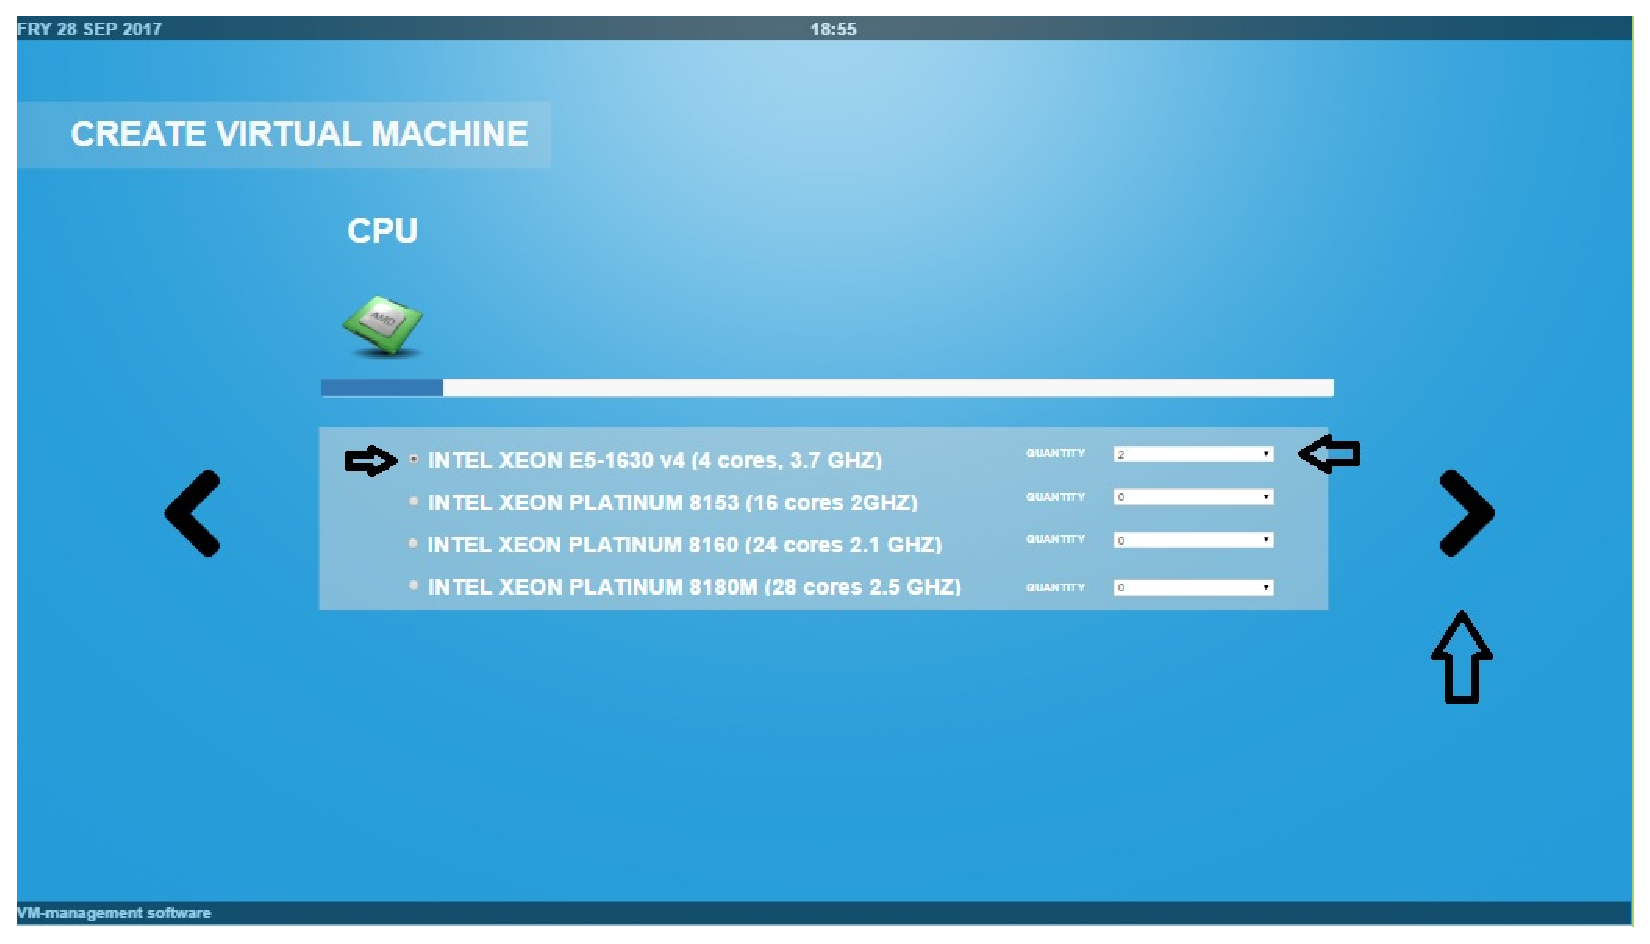
\includegraphics[width=170mm]{images/createVMEx4.eps}
\caption{\label{overflow}}
\end{figure}


\begin{figure}[H]
\centering
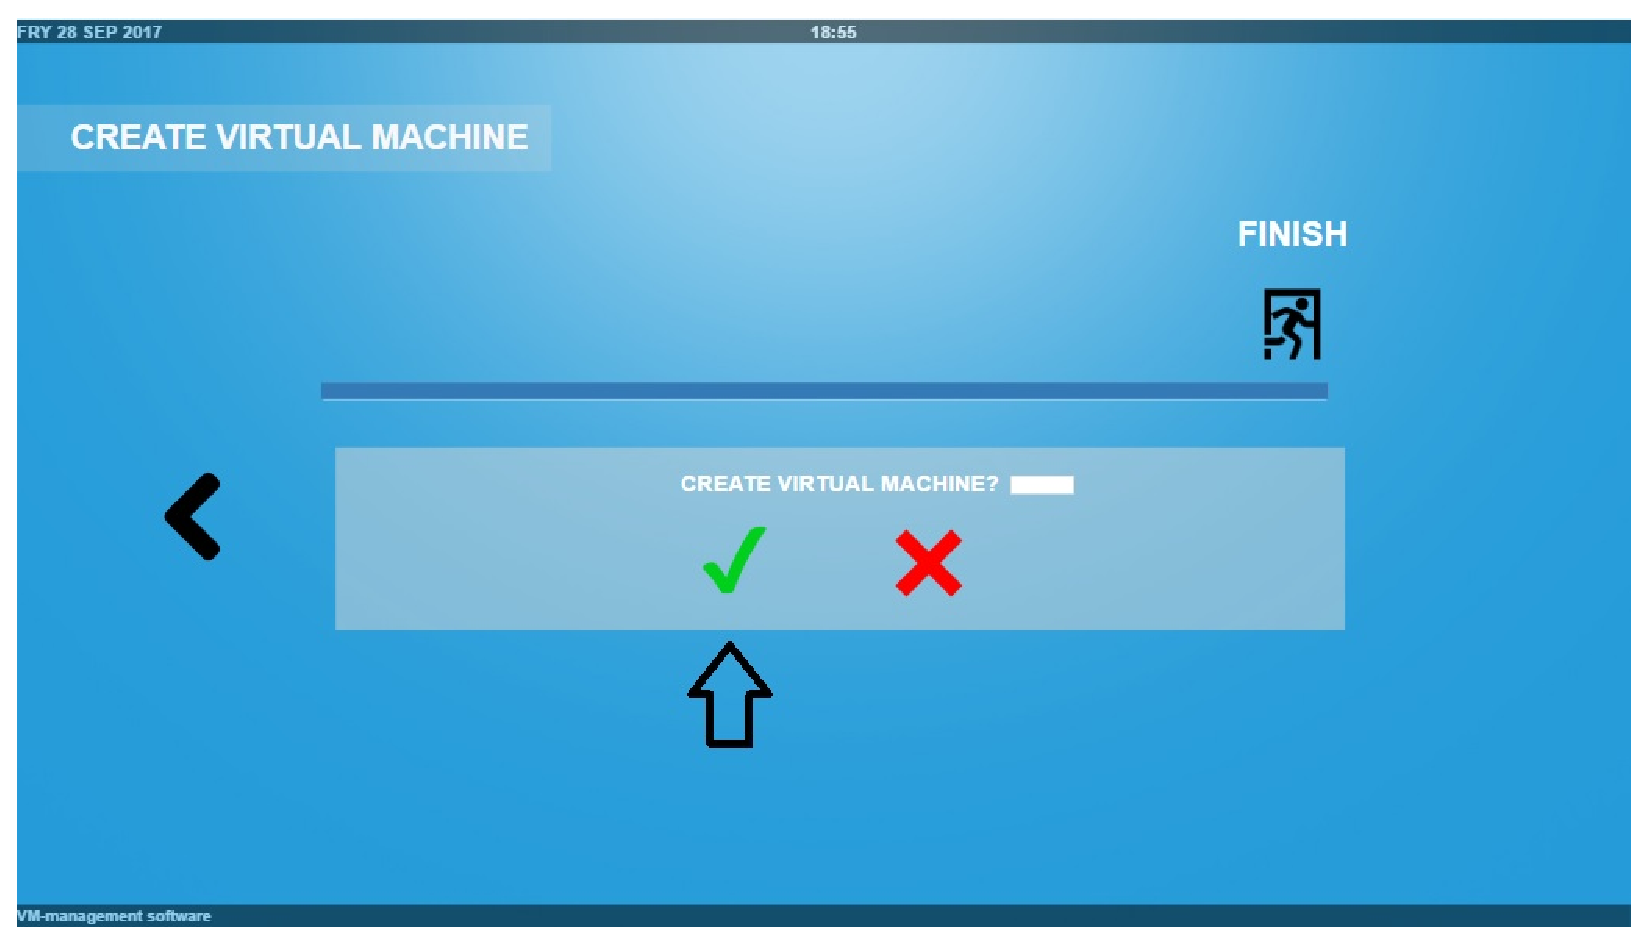
\includegraphics[width=170mm]{images/createVMEx10.eps}
\caption{\label{overflow}}
\end{figure}

\end{lyxlist}
\hrule
\vspace{0.5cm}









\subsubsection{Deleting a virtual machine}

\hrule
\vspace{0.5cm}
\begin{lyxlist}{PC1}
\small{
\item [\textbf{Procedure:}] vmDeletionProcess
\item [\textbf{Scope:}] Virtual machine deletion
\item [\textbf{Primary Actor}:] SysAdmin John 
\item [\textbf{Secondary Actor(s)}:] /
\item [\textbf{Goal:}] The SysAdmin John should be able to delete a virtual
machine which was already created before.
\item [\textbf{Level}:] User-goal level
\item [\textbf{Main~Success~Scenario}]:\\
1. \emph{John} must click on the button "VIEW VM's" in the main Menu.\\
2. \emph{John} will see all the virtual machines that he created.\\
3. \emph{John} must select a virtual machine 'JOHN'sVM'and click on it'.\\
4. \emph{John} must click now on the middle button named `DELETE`.\\
5. \emph{John} must enter his password '1234'.\\
6. \emph{John} must now click on the green check mark to delete the selected
VM.\\



\item [\textbf{Extensions}]:\\
2.a John has to be logged in, in order to create a virtual machine.\\
2.b John must have created at least one virtual machine inorder to perform a
deletion.\\

\item [\textbf{GUI screenshot guide}]:\\
}

\begin{figure}[H]
\centering
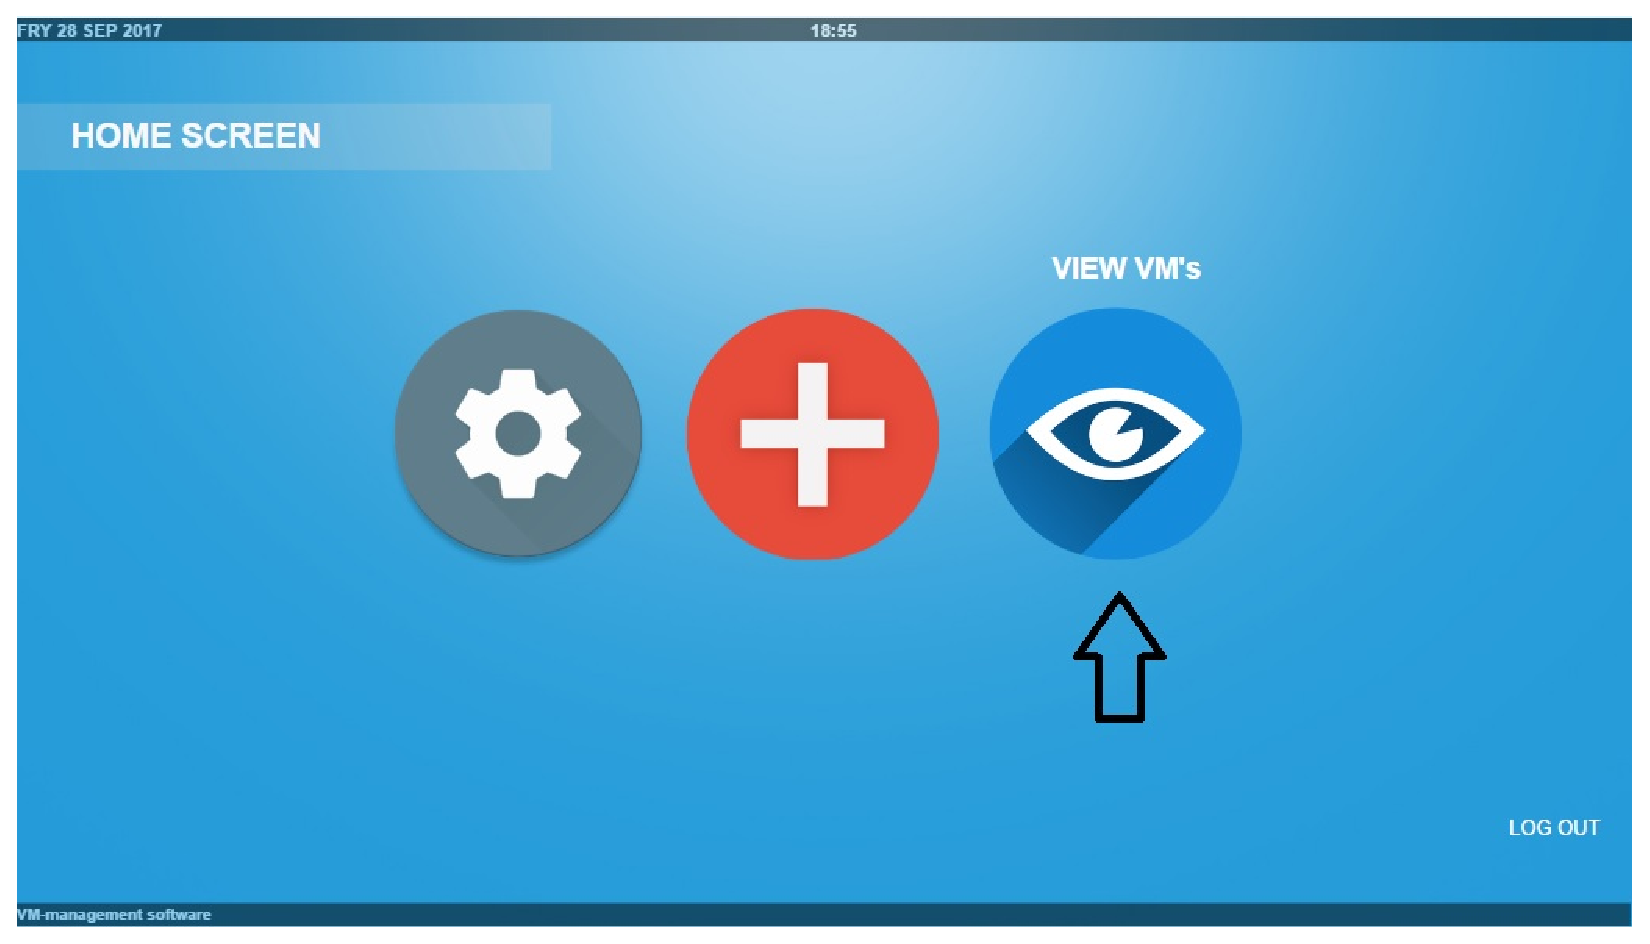
\includegraphics[width=170mm]{images/createVMMod1.eps}
\caption{\label{overflow}}
\end{figure}


\begin{figure}[H]
\centering
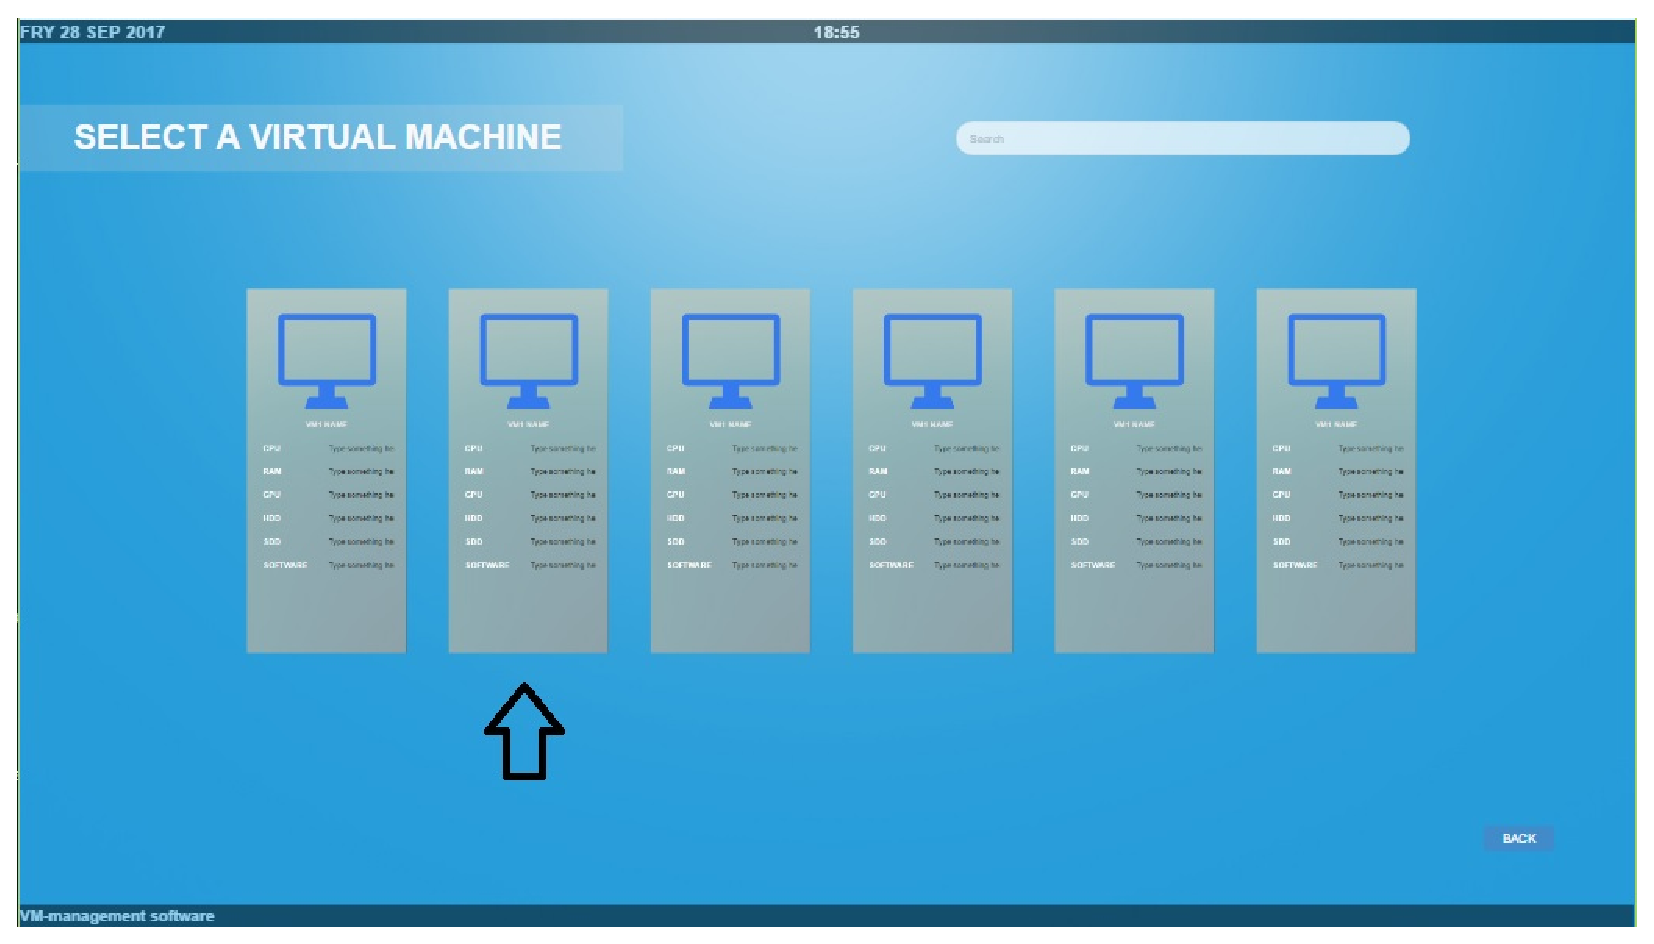
\includegraphics[width=170mm]{images/createVMMod2.eps}
\caption{\label{overflow}}
\end{figure}

\begin{figure}[H]
\centering
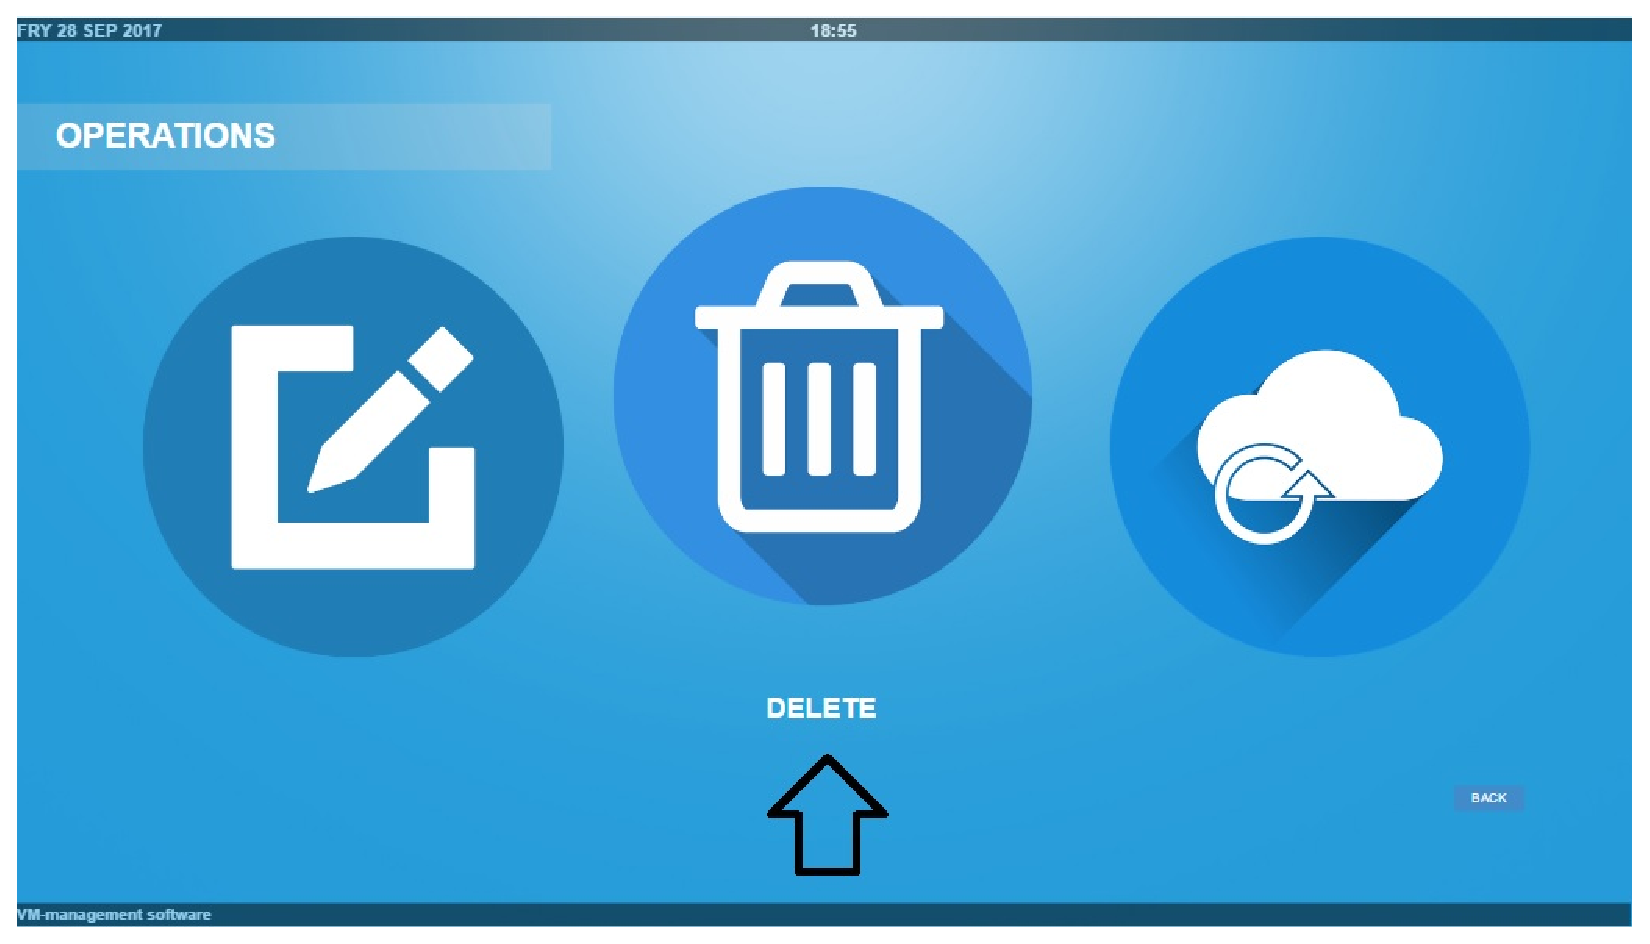
\includegraphics[width=170mm]{images/deleteVM3.eps}
\caption{\label{overflow}}
\end{figure}

\begin{figure}[H]
\centering
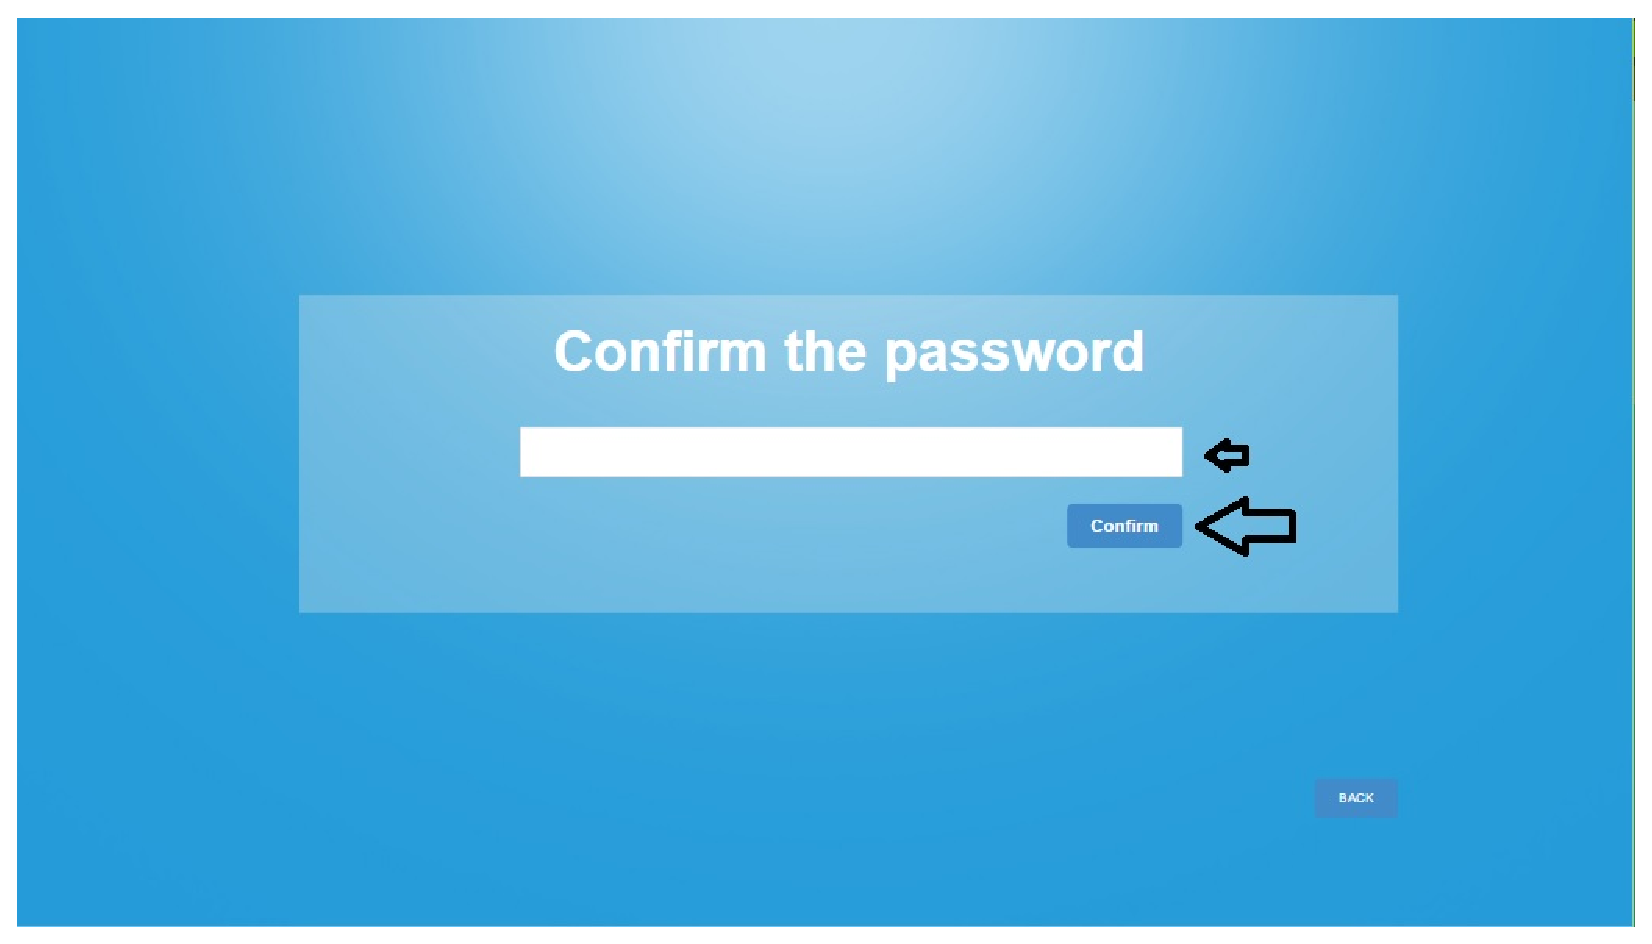
\includegraphics[width=170mm]{images/deleteVM4.eps}
\caption{\label{overflow}}
\end{figure}

\begin{figure}[H]
\centering
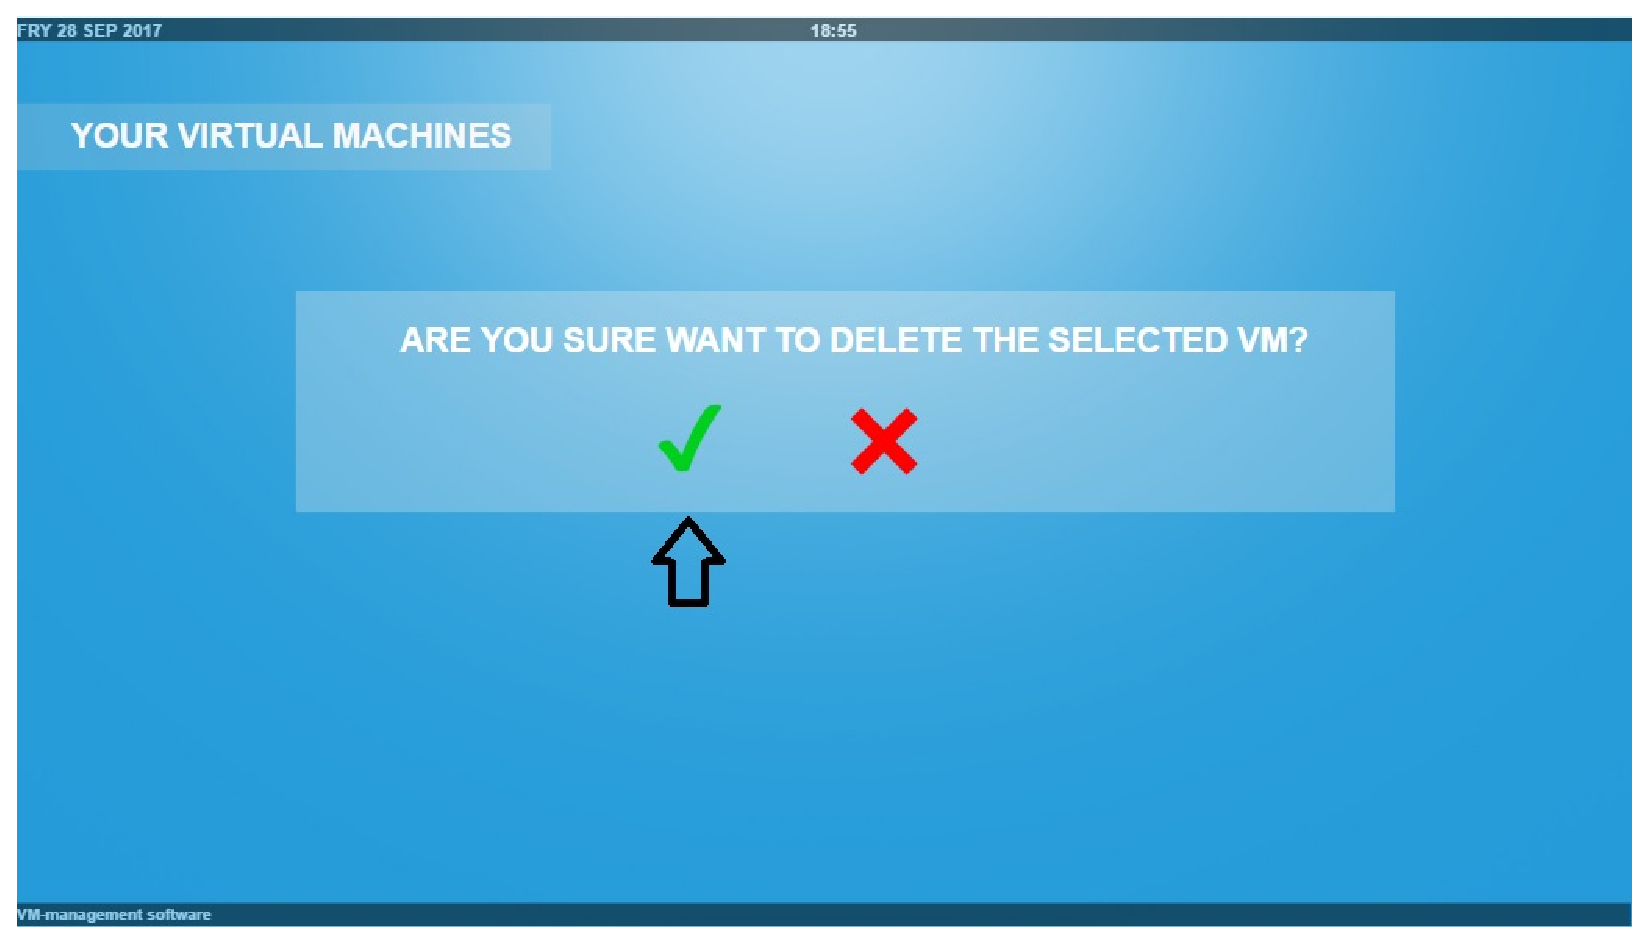
\includegraphics[width=170mm]{images/deleteVM5.eps}
\caption{\label{overflow}}
\end{figure}

\end{lyxlist}
\hrule
\vspace{0.5cm}







\subsubsection{Perform a hot backup}

\hrule
\vspace{0.5cm}
\begin{lyxlist}{PC1}
\small{
\item [\textbf{Procedure:}] vmBackupProcess1
\item [\textbf{Scope:}] Virtual machine backup
\item [\textbf{Primary Actor}:] SysAdmin John 
\item [\textbf{Secondary Actor(s)}:] /
\item [\textbf{Goal:}] The SysAdmin John should be able to perform a hot backup
on a selected virtual machine that John created before.
\item [\textbf{Level}:] User-goal level
\item [\textbf{Main~Success~Scenario}]:\\
1. \emph{John} must click on the button "VIEW VM'S" in the main Menu.\\
2. \emph{John} will see all the virtual machines that he created.\\
3. \emph{John} will select the virtual machine 'JOHN'sVM' on which he wants
to perform a hot backup by clicking on it'.\\
4. \emph{John} must click now on the rightmost button named `BACKUP`.\\
5. \emph{John} must now click on the button named 'BACKUP NOW'.\\
6. \emph{John} must click on the green check mark to accept the requested
operation.\\



\item [\textbf{Extensions}]:\\
2.a John has to be logged in, in order to create a virtual machine.\\
2.b John must have created at least one virtual machine inorder to perform a
hot backup.\\

\item [\textbf{GUI screenshot guide}]:\\
}


\begin{figure}[H]
\centering
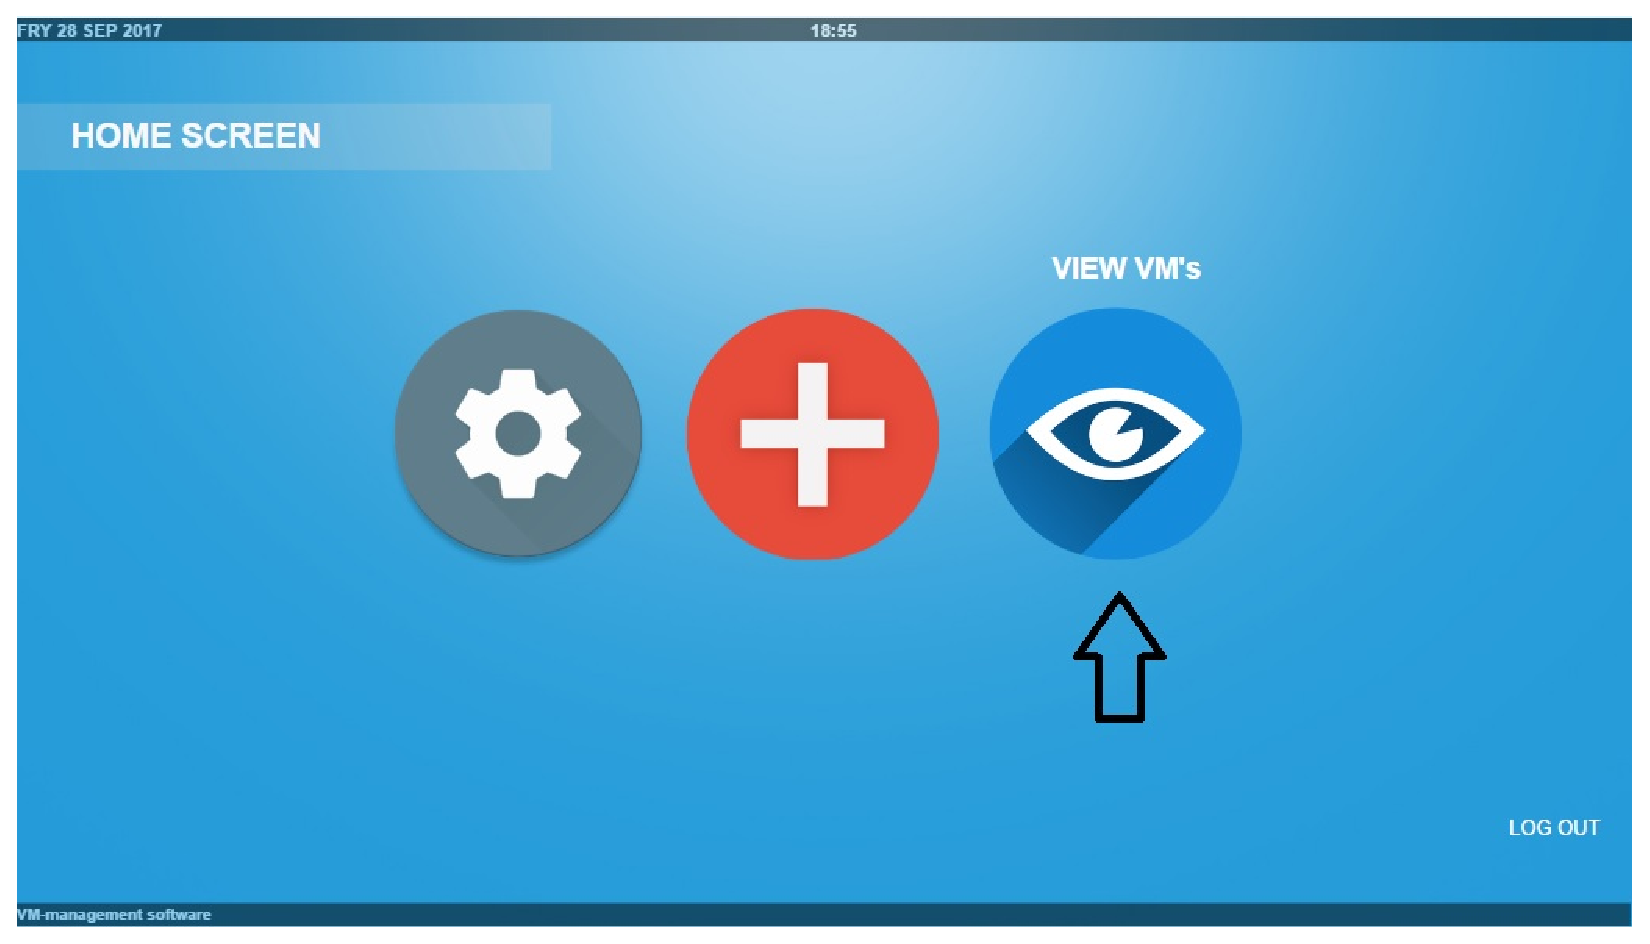
\includegraphics[width=170mm]{images/createVMMod1.eps}
\caption{\label{overflow}}
\end{figure}


\begin{figure}[H]
\centering
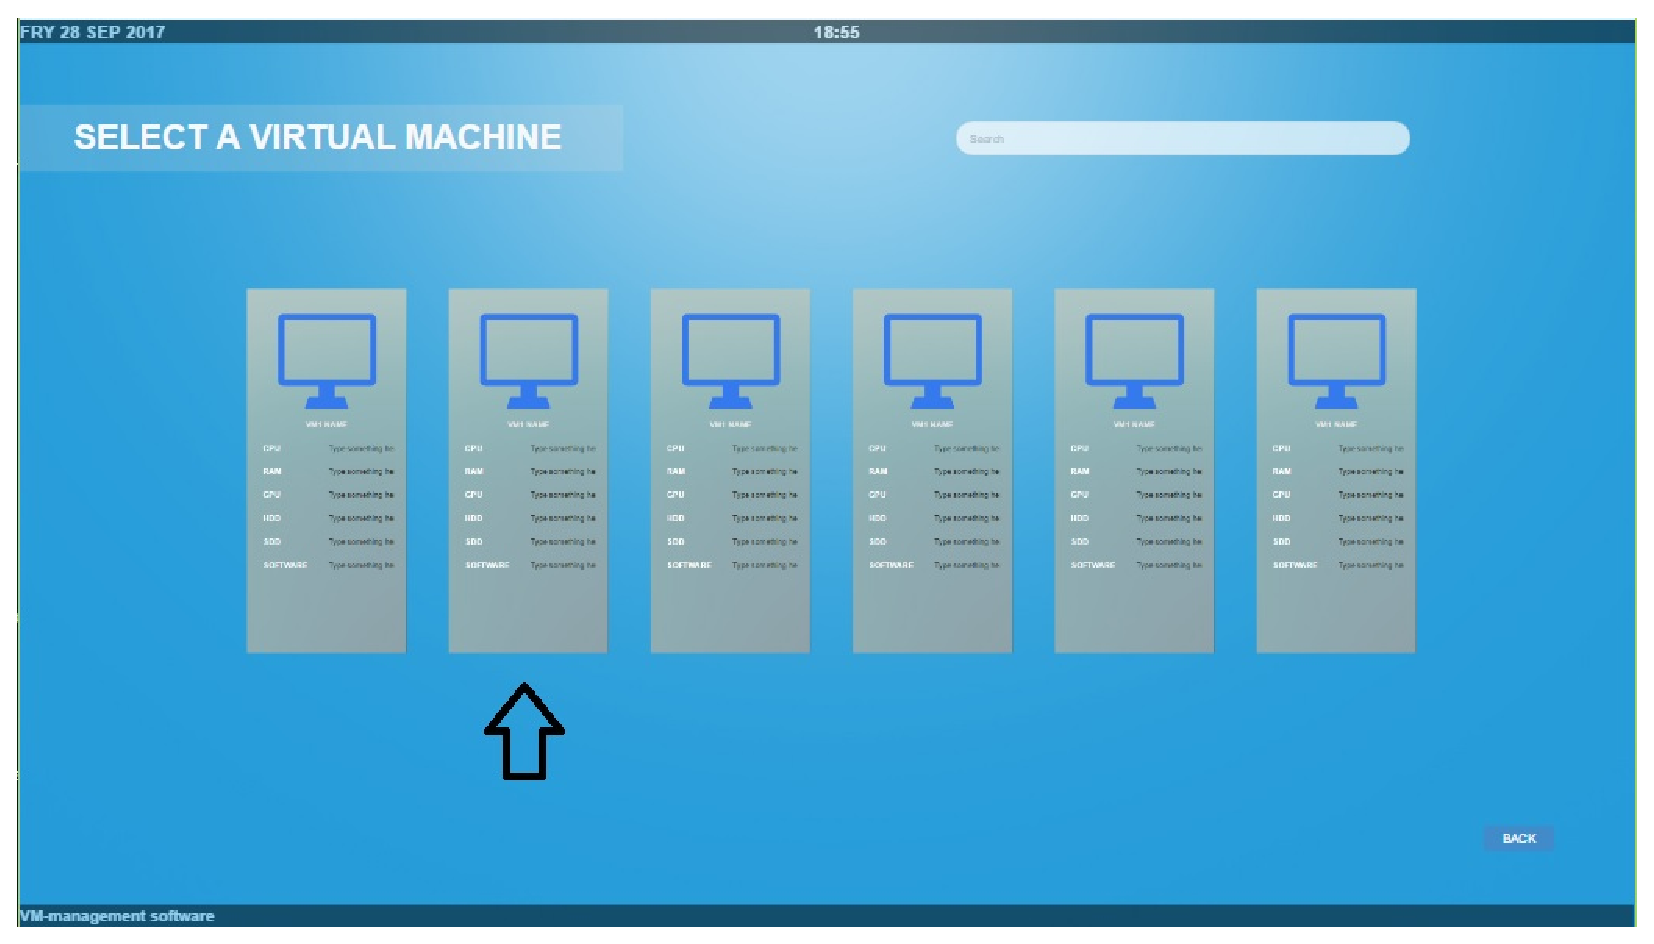
\includegraphics[width=170mm]{images/createVMMod2.eps}
\caption{\label{overflow}}
\end{figure}

\begin{figure}[H]
\centering
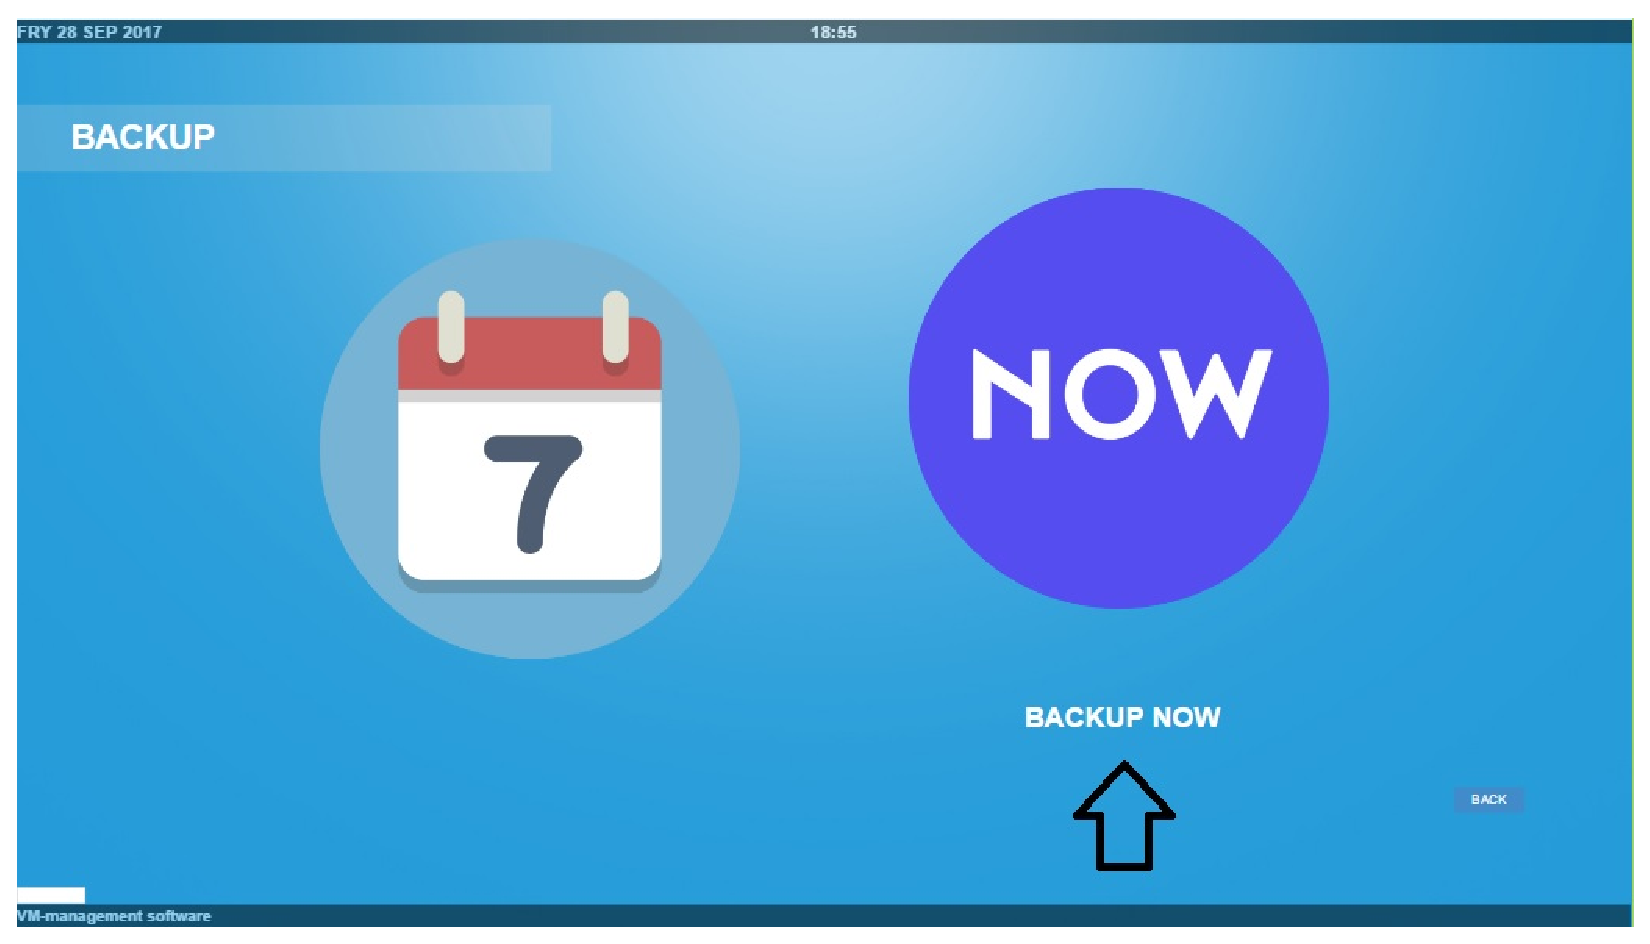
\includegraphics[width=170mm]{images/hotback3.eps}
\caption{\label{overflow}}
\end{figure}

\begin{figure}[H]
\centering
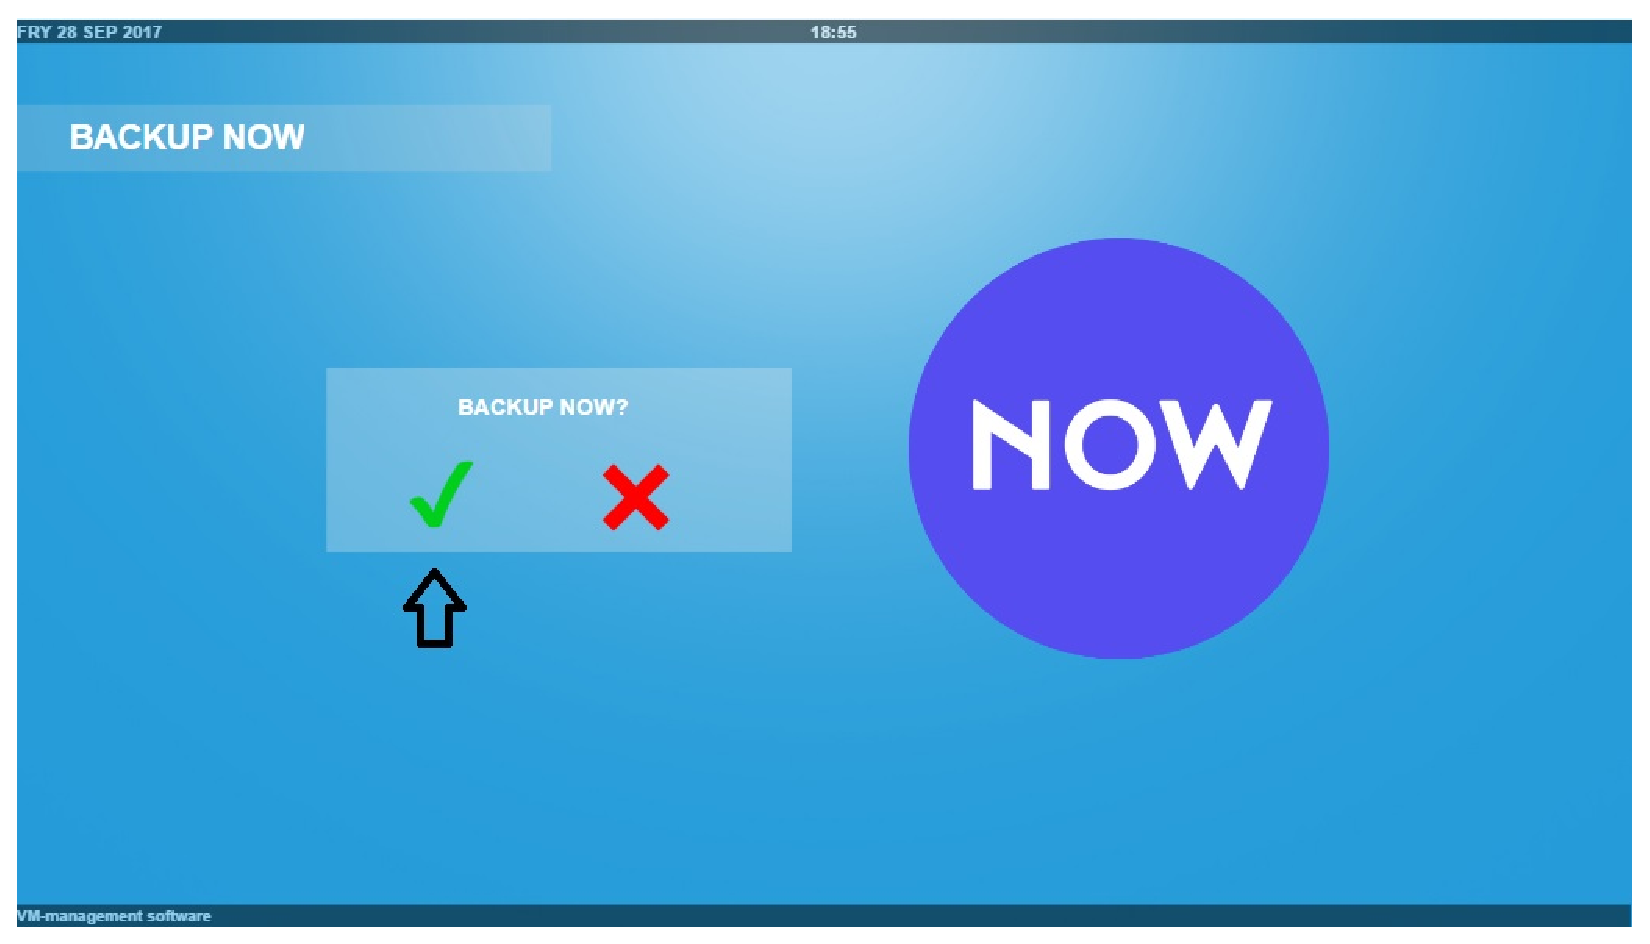
\includegraphics[width=170mm]{images/hotback4.eps}
\caption{\label{overflow}}
\end{figure}

\end{lyxlist}
\hrule
\vspace{0.5cm}










\subsubsection{Perform a scheduled backup}

\hrule
\vspace{0.5cm}
\begin{lyxlist}{PC1}
\small{
\item [\textbf{Procedure:}] vmBackupProcess2
\item [\textbf{Scope:}] Virtual machine backup
\item [\textbf{Primary Actor}:] SysAdmin John 
\item [\textbf{Secondary Actor(s)}:] /
\item [\textbf{Goal:}] The SysAdmin John should be able to perform a
scheduled backup on a selected virtual machine that John created before.
\item [\textbf{Level}:] User-goal level
\item [\textbf{Main~Success~Scenario}]:\\
1. \emph{John} must click on the button "VIEW VM's" in the main
Menu.\\
2. \emph{John} will see all the virtual machines that he created.\\
3. \emph{John} will select the virtual machine 'JOHN'sVM' on which he wants
to perform a scheduled backup by clicking on it'.\\
4. \emph{John} must click now on the rightmost button named `BACKUP`.\\
5. \emph{John} must now click on the button named 'SCHEDULED
BACKUP'.\\
6. \emph{John} will add a small description in the description label such as
'Backup for version 0.3 of sofware engeneering project.\\
7. \emph{John} must specify a date '15/10/2017' by clicking on the calender on a
specific day.\\
8. \emph{John} must click on the button named 'PERFORM' to perform the backup.\\



\item [\textbf{Extensions}]:\\
2.a John has to be logged in, in order to create a virtual machine.\\
2.b John must have created at least one virtual machine inorder to perform a
cold/scheduled backup.\\

\item [\textbf{GUI screenshot guide}]:\\
}


\begin{figure}[H]
\centering
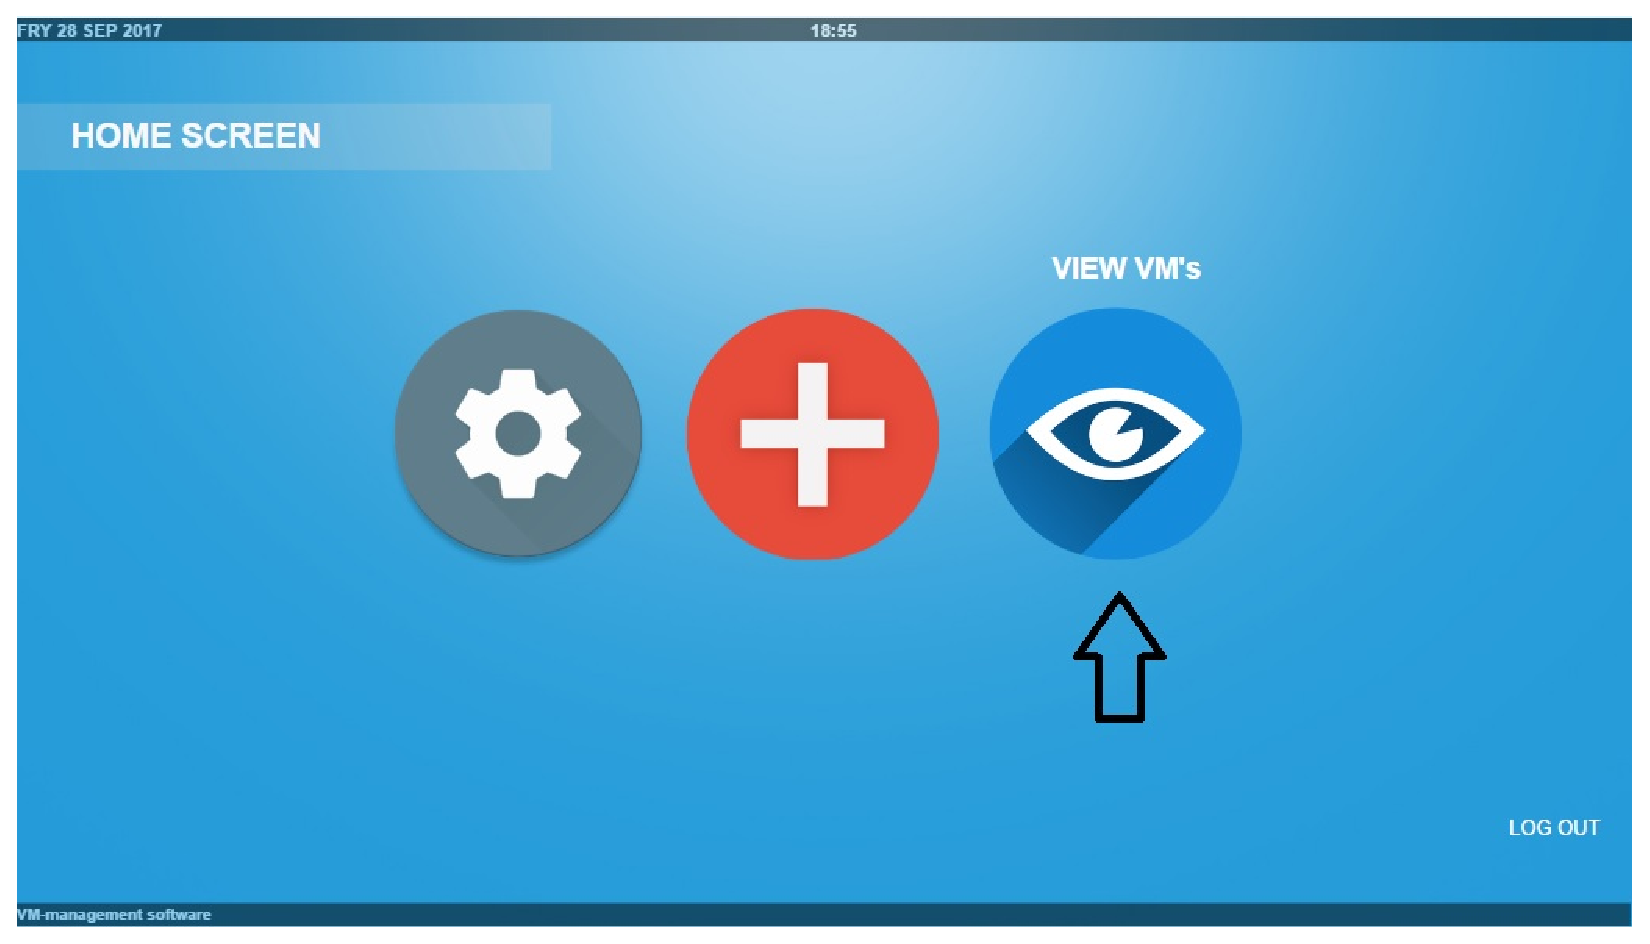
\includegraphics[width=170mm]{images/createVMMod1.eps}
\caption{\label{overflow}}
\end{figure}


\begin{figure}[H]
\centering
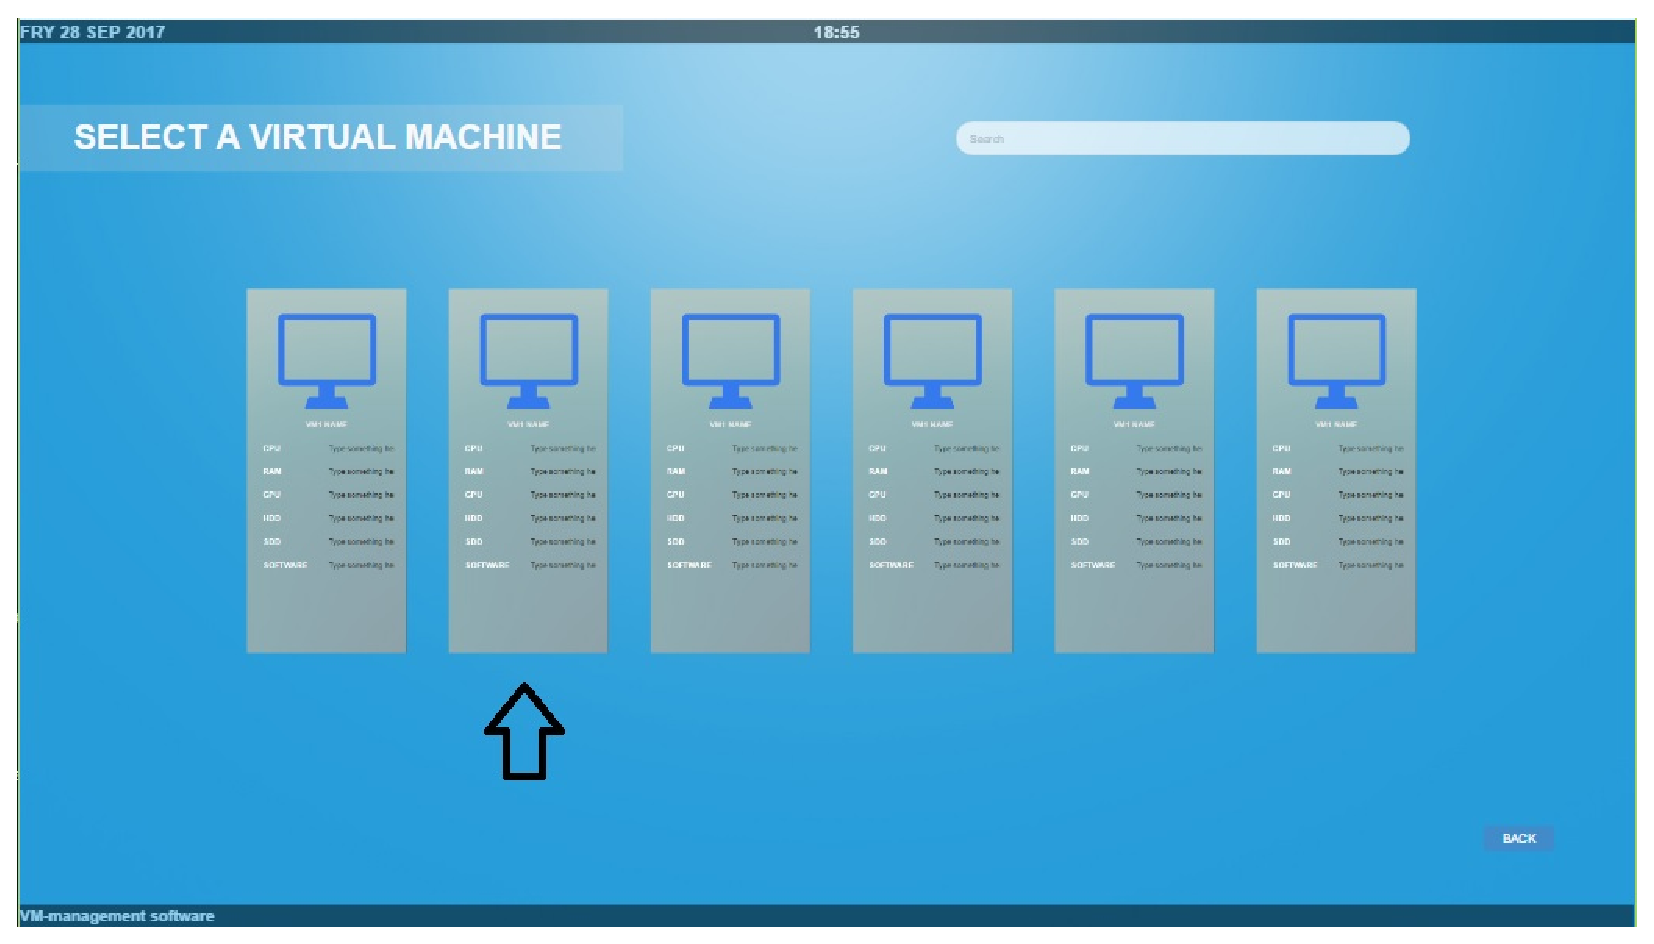
\includegraphics[width=170mm]{images/createVMMod2.eps}
\caption{\label{overflow}}
\end{figure}

\begin{figure}[H]
\centering
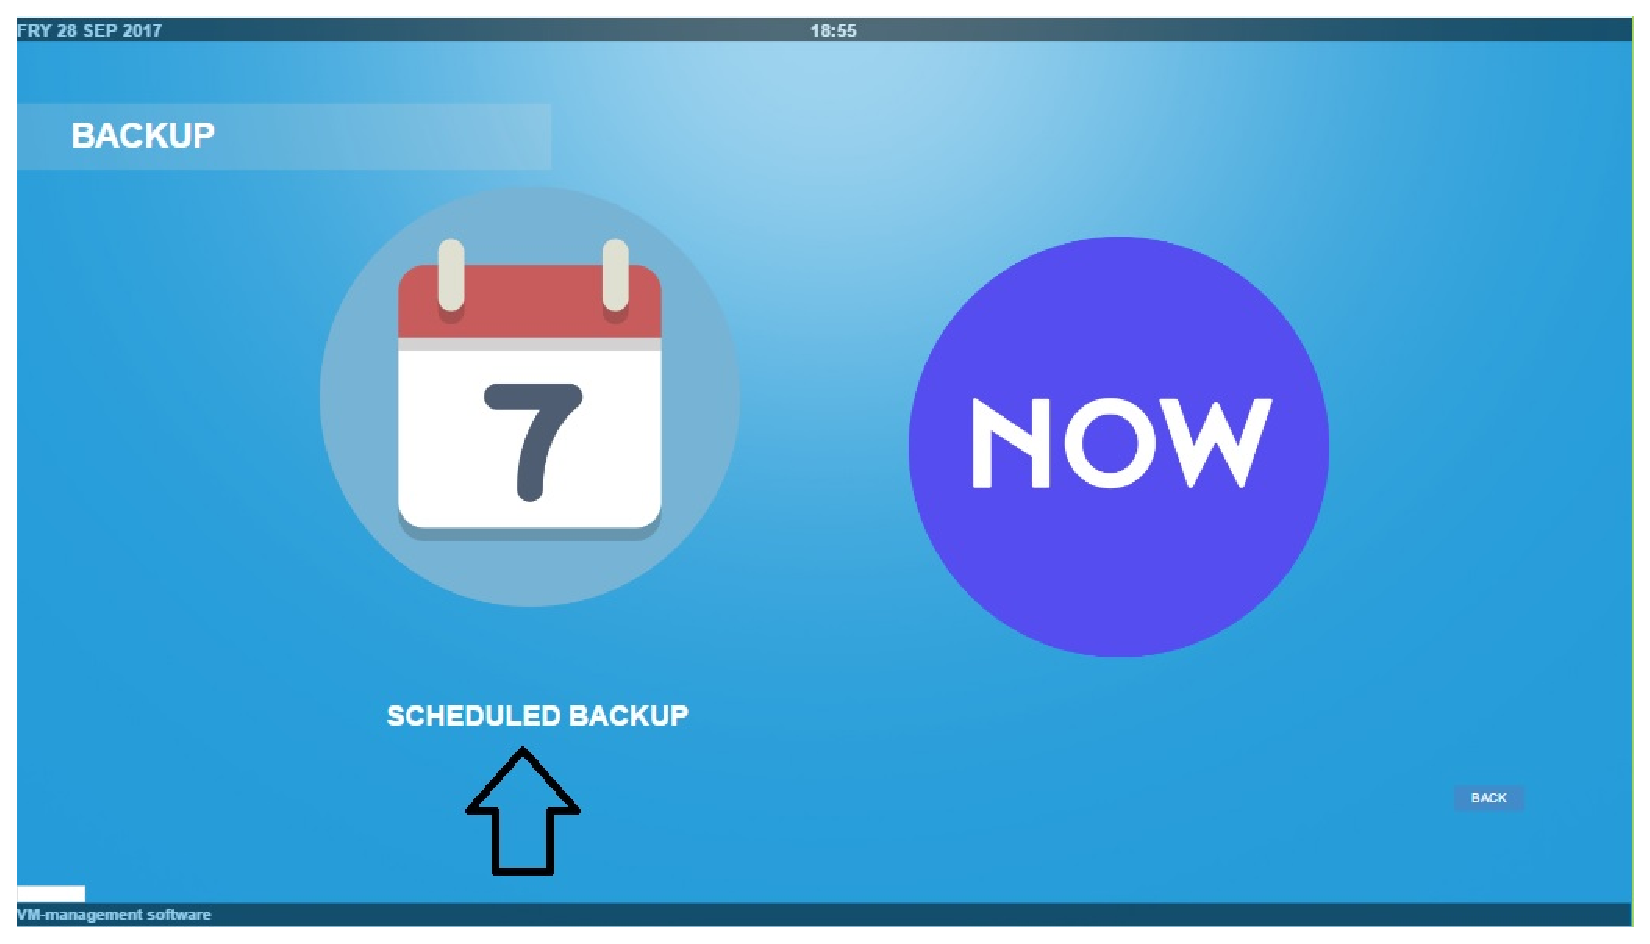
\includegraphics[width=170mm]{images/schback3.eps}
\caption{\label{overflow}}
\end{figure}


\begin{figure}[H]
\centering
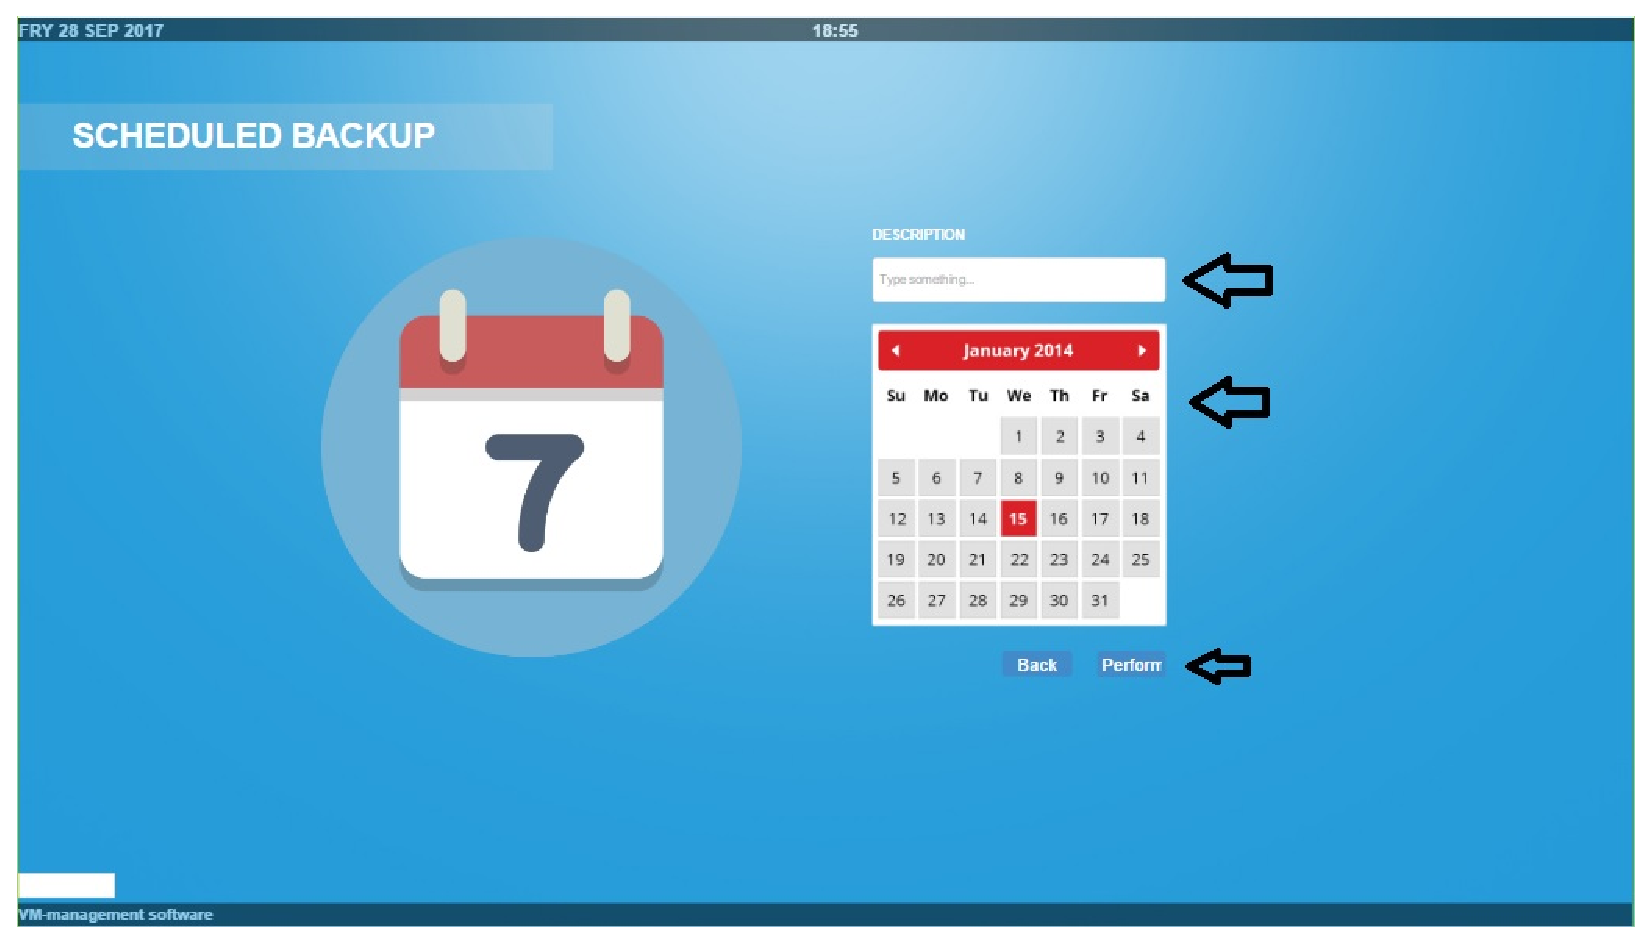
\includegraphics[width=170mm]{images/schback4.eps}
\caption{\label{overflow}}
\end{figure}

\end{lyxlist}
\hrule
\vspace{0.5cm}


\subsubsection{Delete Account}

\hrule
\vspace{0.5cm}
\begin{lyxlist}{PC1}
\small{
\item [\textbf{Procedure:}] DeleteAccount 
\item [\textbf{Scope:}] Allow the the SysAdmin to delete his account.
\item [\textbf{Primary Actor}:] SysAdmin Tom
\item [\textbf{Secondary Actor(s)}:] /
\item [\textbf{Goal:}] The SysAdmin Tom should be able to delete his account.
\item [\textbf{Level}:] User-goal level
\item [\textbf{Main~Success~Scenario}]:\\
1. \emph{Tom} clicks on the "Delete Account'' icon in the Password settings
section.\\
2. \emph{Tom} inserts his password in the input text field.\\
3. \emph{Tom} clicks on the ''Confirm'' button to confirm the password.\\
4. \emph{Tom} clicks on the ''YES'' button(if he really wants to delete his
acount.) or clicks on ''NO'' button(if he don't want to delete his account).\\
5. \emph If {Tom} clicked on the "YES" button, the account is deleted and
{Tom} clicks on the "ok" button to terminate the procedure.\\
6. \emph If {Tom} clicked on the "NO" button, the account is not deleted.\\

\item [\textbf{Extensions}]:\\
2.a \emph{Tom} has to be a SysAdmin and has to be logged in in order to be able
to delete his account.\\
}


\begin{figure}[H]
\centering
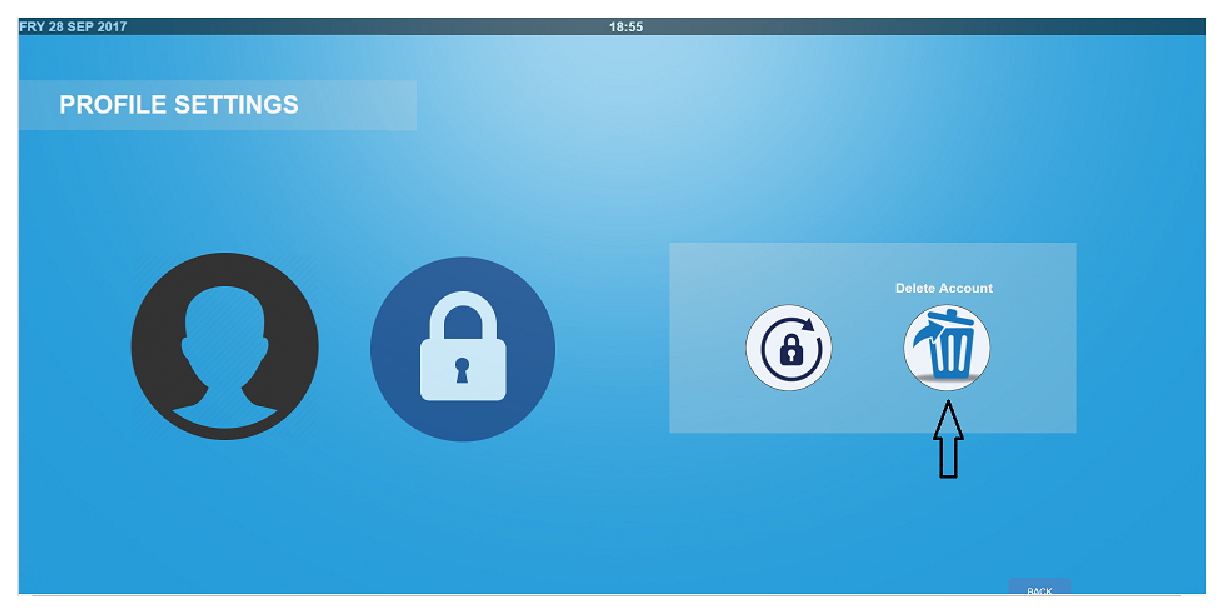
\includegraphics[width=170mm]{images/deletAcc1.eps}
\caption{\label{overflow}}
\end{figure}


\begin{figure}[H]
\centering
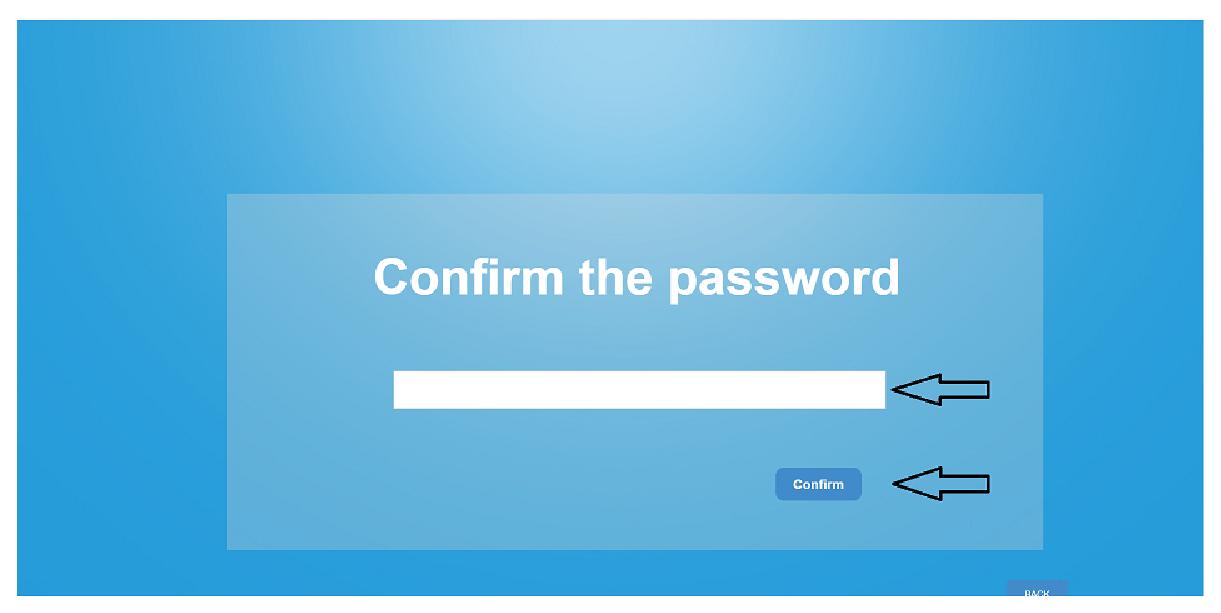
\includegraphics[width=170mm]{images/ComfirmField.eps}
\caption{\label{overflow}}
\end{figure}


\begin{figure}[H]
\centering
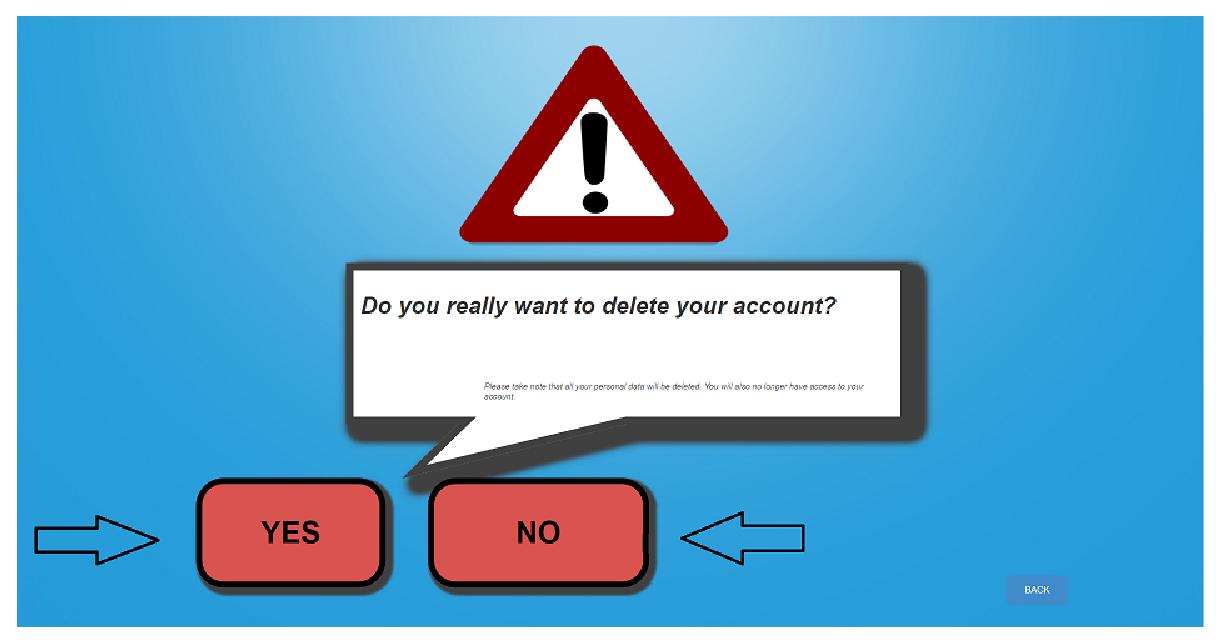
\includegraphics[width=170mm]{images/deletAcc2.eps}
\caption{\label{overflow}}
\end{figure}



\end{lyxlist}
\hrule




\subsection{super-SysAdmin}

\subsubsection{Overview of the datacenter}

\hrule
\vspace{0.5cm}
\begin{lyxlist}{PC1}
\small{
\item [\textbf{Procedure:}] DatacenterOverview
\item [\textbf{Scope:}] Datacenter Management
\item [\textbf{Primary Actor}:] super-SysAdmin Bob
\item [\textbf{Secondary Actor(s)}:] /
\item [\textbf{Goal:}] The super-SysAdmin Bob should be able to get an overview
of the datacenter
\item [\textbf{Level}:] User-goal level
\item [\textbf{Main~Success~Scenario}]:\\
1. \emph{Bob} has to click on the \emph{Hardware} button in the home screen.\\
2. \emph{Bob} has the choice to overview a component individually.\\
3. \emph{Bob} clicks on the \emph{CPU} icon to get the usage overview of the
CPU.\\
4. To see another component's overview \emph{Bob} clicks on the \emph{SSD}
icon.\\


\item [\textbf{Extensions}]:\\
2.a \emph{Bob} has to be an super-SysAdmin and has to be logged in in order to
be able to overview the datacenter's usage.\\

\item [\textbf{GUI screenshot guide}]:\\
}


\begin{figure}[H]
\centering
\includegraphics[width=170mm]{images/overviewComponent1.eps}
\caption{\label{overflow}}
\end{figure}


\begin{figure}[H]
\centering
\includegraphics[width=170mm]{images/overviewComponent2.eps}
\caption{\label{overflow}}
\end{figure}


\begin{figure}[H]
\centering
\includegraphics[width=170mm]{images/overviewComponent3.eps}
\caption{\label{overflow}}
\end{figure}

\end{lyxlist}
\hrule
\vspace{0.5cm}


\subsubsection{Request new component(s)}

\hrule
\vspace{0.5cm}
\begin{lyxlist}{PC1}
\small{
\item [\textbf{Procedure:}] ComponentRequest
\item [\textbf{Scope:}] Request of a/multiple component(s)
\item [\textbf{Primary Actor}:] super-SysAdmin Bob
\item [\textbf{Secondary Actor(s)}:] /
\item [\textbf{Goal:}] The super-SysAdmin Bob should be able to request new
component(s)
\item [\textbf{Level}:] User-goal level
\item [\textbf{Main~Success~Scenario}]:\\
1. \emph{Bob} has to click on the \emph{Harware} button in the home screen.\\
2. \emph{Bob} clicks on the \emph{Request Component} button.\\
3. \emph{Bob} clicks on CPU's model button \emph{INTEL XEON E5-1360
v4(4cores, 3.7 GHz)}.\\
4. \emph{Bob} selects the quantity as 2.\\
5. \emph{Bob} clicks on CPU's model button \emph{INTEL XEON PLATINUM 8160
(24 cores, 2.1 GHz)}.\\
6. \emph{Bob} selects the quantity as 2.\\
7. \emph{Bob} clicks on RAM's model button \emph{16GB ECC Memory}.\\
8. \emph{Bob} selects the quantity as 1.\\
9. \emph{Bob} clicks on RAM's model button \emph{32GB ECC Memory}.\\
10. \emph{Bob} selects the quantity as 3.\\
11. \emph{Bob} clicks on HDD's model button \emph{32TB 7200 RPM}.\\
12. \emph{Bob} selects the quantity as 3.\\
13. \emph{Bob} clicks on HDD's model button \emph{64TB 7200 RPM}.\\
14. \emph{Bob} selects the quantity as 5.\\
15. \emph{Bob} clicks on SSD's model button \emph{1TB SATA SSD}.\\
16. \emph{Bob} selects the quantity as 4.\\
17. \emph{Bob} clicks on SSD's model button \emph{1TB NVME M.2 SSD}.\\
18. \emph{Bob} selects the quantity as 2.\\
19. \emph{Bob} clicks on SSD's model button \emph{2TB NVME M.2 SSD}.\\
20. \emph{Bob} selects the quantity as 3.\\
21. \emph{Bob} clicks on SSD's model button \emph{4TB NVME M.2 SSD}.\\
22. \emph{Bob} selects the quantity as 2.\\
23. \emph{Bob} clicks on Software's model button \emph{SOLIDWORKS 2017}.\\
24. \emph{Bob} selects the quantity as 4.\\
25. \emph{Bob} clicks on the \emph{Next} button.\\
26. \emph{Bob} clicks on the \emph{Yes} button to confirm that the request
is send.\\

\item [\textbf{Extensions}]:\\
2.a \emph{Bob} has to be an super-SysAdmin and has to be logged in in order to
be able to request a new component(s).\\

\item [\textbf{GUI screenshot guide}]:\\
}


\begin{figure}[H]
\centering
\includegraphics[width=170mm]{images/requestComponent1.eps}
\caption{\label{overflow}}
\end{figure}

\begin{figure}[H]
\centering
\includegraphics[width=170mm]{images/requestComponent2.eps}
\caption{\label{overflow}}
\end{figure}

\begin{figure}[H]
\centering
\includegraphics[width=170mm]{images/requestComponent3.eps}
\caption{\label{overflow}}
\end{figure}

\begin{figure}[H]
\centering
\includegraphics[width=170mm]{images/requestComponent4.eps}
\caption{\label{overflow}}
\end{figure}

\end{lyxlist}
\hrule
\vspace{0.5cm}






\subsubsection{Creating a SysAdmin}

\hrule
\vspace{0.5cm}
\begin{lyxlist}{PC1}
\small{
\item [\textbf{Procedure:}] SysAdminCreation 
\item [\textbf{Scope:}] Allow the super administrator to create a new SysAdmin
\item [\textbf{Primary Actor}:] super-SysAdmin Bob
\item [\textbf{Secondary Actor(s)}:] /
\item [\textbf{Goal:}] The super-SysAdmin Bob should be able to create a new
regular user.
\item [\textbf{Level}:] User-goal level
\item [\textbf{Main~Success~Scenario}]:\\
1. \emph{Bob} has to click on the "CREATE NEW USER '' button in the super-SysAdmin home
screen.\\
2. \emph{Bob} has to fill the different textfields.\\
3. \emph After the different texfields have been filled. {Bob} has to click on
the "next step" button.\\
4. \emph{Bob} has to attribute the different rights for the SysAdmin.
{Bob} need only to click in the litle box if he want to attribute a right.\\
5. \emph{Bob} only needs now to click on the ``Create user" button for create a
SysAdmin.
\\
6. \emph A new SysAdmin has been created and {Bob} only needs to click
on the " ok" button.\\

\item [\textbf{Extensions}]:\\
2.a \emph{Bob} has to be an super-SysAdmin and has to be logged in in order to
be able to create a sysAdmin.\\
}

\begin{figure}[H]
\centering
\includegraphics[width=170mm]{images/CreateSys11.eps}
\caption{\label{overflow}}
\end{figure}

\begin{figure}[H]
\centering
\includegraphics[width=170mm]{images/CreateSys2.eps}
\caption{\label{overflow}}
\end{figure}

\begin{figure}[H]
\centering
\includegraphics[width=170mm]{images/CreateSys3.eps}
\caption{\label{overflow}}
\end{figure}

\begin{figure}[H]
\centering
\includegraphics[width=170mm]{images/CreateSys4.eps}
\caption{\label{overflow}}
\end{figure}
\end{lyxlist}
\hrule

















